%!TEX root = /Users/louis/Documents/PhD/Deliverables/Thesis/thesis.tex

\chapter{Design and Implementation}
\label{Implementation}
Section~\ref{sec:requirements_identification} presented requirements for structures and processes for identifying and managing co-evolution. This chapter describes the way in which the requirements have been addressed. Several related structures have been implemented, using domain-specific languages, metamodelling and model management operations. Figure~\ref{fig:implementation_overview} summarises the contents of the chapter. To facilitate the management of non-conformant models with existing modelling frameworks, a metamodel-independent syntax was devised and implemented (Section~\ref{sec:mmi_syntax}). To address some of the challenges faced in user-driven co-evolution, an OMG specification for a textual modelling notation was implemented (Section~\ref{sec:notation}). Finally, a model transformation language -- tailored for model migration and centred around a novel approach to relating source and target model elements -- was designed and implemented (Sections~\ref{sec:analyis_of_languages_used_for_migration} and~\ref{sec:flock}). 

\begin{figure}[htbp]
  \begin{center}
    \leavevmode
    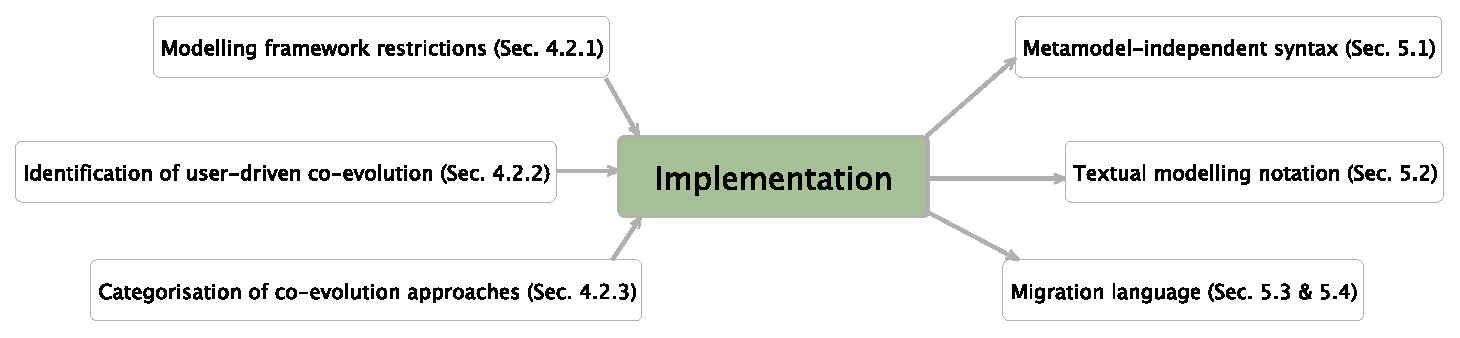
\includegraphics[width=12cm]{5.Implementation/overview.pdf}
  \end{center}
  \caption{Implementation chapter overview.}
  \label{fig:implementation_overview}
\end{figure}

The structures presented in this chapter are interoperable as shown in Figure~\ref{fig:implementation_structure}. In particular, the modelling framework extensions provided by the metamodel-independent syntax are used to provide conformance checking for the textual modelling notation, and to enable conformance checking for the model migration language. The structures were separated to facilitate re-use of the conformance checking services provided by the metamodel-independent syntax. Table~\ref{tab:implementation_to_requirements} shows the relationship between the proposed structures and the thesis requirements (Section~\ref{sec:requirements_identification}).

\begin{figure}[htbp]
	\centering
		\includegraphics*[viewport=0 400 800 800,height=5cm]{5.Implementation/images/implementation_structure.pdf}
	\caption{The relationships between the proposed structures}
	\label{fig:implementation_structure}
\end{figure}

\begin{table}[tbhp]
	\centering
	\begin{tabular}{|c|l|}
		\hline
		\textbf{Structure (Section)} & \textbf{Requirement} \\
		\hline
		\multirow{6}{*}{Metamodel-independent syntax (\ref{sec:mmi_syntax})} & This thesis must investigate the \\
		& extension of existing modelling \\ 
		& frameworks to support the loading \\
		& of non-conformant models and \\
		& conformance checking of models \\
		& against other metamodels. \\
		\hline
		\multirow{9}{*}{Textual modelling notation (\ref{sec:notation})} & This thesis must demonstrate a \\
		& user-driven co-evolution process \\
		& that enables the editing of \\
		& non-conformant models without \\
		& directly manipulating the \\
		& underlying storage representation \\
		& and provides a conformance report \\
		& for the original model and \\
		& evolved metamodel. \\
		\hline
		\multirow{4}{*}{Model migration language (\ref{sec:analyis_of_languages_used_for_migration})} & This thesis must compare and \\
    & evaluate existing languages \\
		& for specifying model   \\
		& migration strategies.  \\
		\hline
		\multirow{7}{*}{Model migration language (\ref{sec:flock})} & This thesis must implement and \\
		& evaluate a domain-specific \\
		& language for specifying and \\
		& executing model migration \\
		& strategies, comparing it to \\
		& existing languages for specifying \\ 
		& model migration strategies. \\
		\hline
	\end{tabular}
	\caption{The relationship between the thesis requirements and the proposed structures.}
	\label{tab:implementation_to_requirements}
\end{table}

%!TEX root = /Users/louis/Documents/PhD/Deliverables/Thesis/thesis.tex

% TODO - present MM independent syntax. Make clear that it is an ABSTRACT syntax.

% TODO - Consider discussing the number of revisions of say, UML (and other metamodels), in Chapter 2. This will allow the reader to get a sense of the scale of the problem.

\section{A Metamodel-Independent Syntax}
\label{sec:mmi_syntax}
Section~\ref{subsec:modelling_framework_characteristics} discussed the way in which modelling frameworks implicitly enforce conformance, and hence prevent the loading of non-conformant models. Additionally, modelling frameworks provide little support for checking the conformance of a model with other versions of a metamodel, which is potentially useful during metamodel installation. In Section~\ref{sec:requirements_identification}, these concerns lead to the identification of the following requirement: \emph{This thesis must investigate the extension of existing modelling frameworks to support the loading of non-conformant models and conformance checking of models against other metamodels.}

This section describes the way in which existing modelling frameworks load and store models using metamodel-specific binding mechanisms, proposes an alternative binding mechanism using a metamodel-independent syntax, and demonstrates how this facilitates automatic consistency checking. The work presented in this section has been published in \cite{rose09enhanced}.

\begin{figure}[htbp]
	\centering
	\subfigure[Original metamodel.]
	{
	    \label{fig:original_families_mm}
	    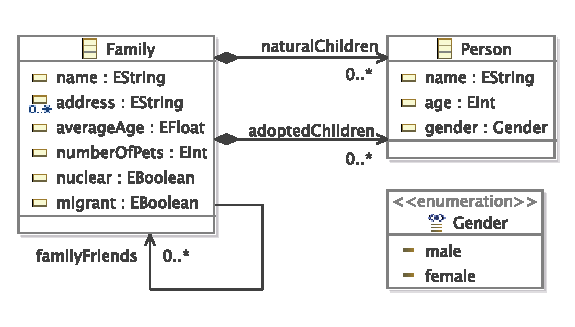
\includegraphics[scale=0.9]{5.Implementation/images/families.pdf}
	}
	\subfigure[Evolved metamodel.]
	{
	    \label{fig:evolved_families_mm}
	    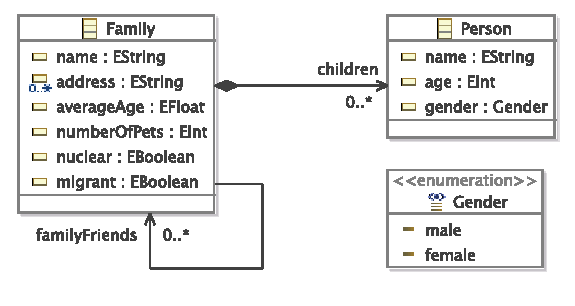
\includegraphics[scale=0.9]{5.Implementation/images/families_evolved.pdf}
	}
	\caption{Evolution of a families metamodel, based on the metamodel in \cite{hutn}.}
\label{fig:families_mms}
\end{figure}

\subsection{Metamodel Evolution Example: Families}
\label{subsec:families_example}
This section uses the example of metamodel evolution in Figure~\ref{fig:families_mms}. The metamodels in Figure~\ref{fig:families_mms} have been constructed in Ecore, the metamodelling language of EMF, which is based on MOF (Section~\ref{subsec:mof}). The metamodels use Ecore types such as \texttt{ESt\-ri\-ng} and \texttt{EFlo\-at}. The \texttt{nu\-cl\-e\-ar} attribute on the \texttt{Fa\-mi\-ly} type is used to indicate that the family ``comprises only a father, a mother, and children.'' \cite{nucleardef}, and not extended family members (such as cousins or grandparents).

In Figure~\ref{fig:original_families_mm}, \texttt{na\-tu\-r\-alCh\-il\-dr\-en} and \texttt{ad\-op\-t\-edCh\-il\-dr\-en} are modelled as separate features, and, in Figure~\ref{fig:evolved_families_mm}, they are modelled as a single feature, \texttt{ch\-il\-dr\-en}. Models that specify values for the \texttt{na\-tu\-r\-alCh\-il\-dr\-en} or \texttt{ad\-op\-t\-edCh\-il\-dr\-en} features do not conform to the evolved metamodel. For example, the model in Figure~\ref{fig:families_model} represents a \texttt{Fa\-mi\-ly} comprising two \texttt{Pe\-rs\-on}s, conforms to the original metamodel, and does not conform to the evolved metamodel. Using the families metamodel and model, the sequel explains why existing modelling frameworks cannot be used to load non-conformant models.

\begin{figure}[htbp]
  \begin{center}
    \leavevmode
    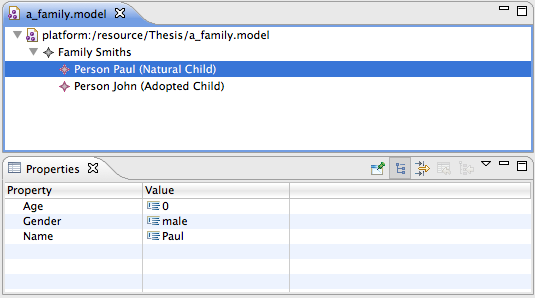
\includegraphics[width=10cm]{5.Implementation/images/family_model.png}
  \end{center}
  \caption[A family model]{A family model, which conforms to the metamodel in Figure~\ref{fig:original_families_mm}}
  \label{fig:families_model}
\end{figure}


\subsection{Binding to a Specific Metamodel}
\label{subsec:binding_specific}
To load a model, existing modelling frameworks construct objects in the underlying programming language in a process termed \emph{binding} (Section~\ref{subsec:modelling_framework_characteristics}). The metamodel defines the way in which model elements will be bound, and binding is strongly-typed. Figure~\ref{fig:successful_binding} illustrates the results of binding the family model in Figure~\ref{fig:families_model} to the original families metamodel in Figure~\ref{fig:original_families_mm}. The objects in Figure~\ref{fig:successful_binding} instantiate types that are defined in the metamodel, such as \texttt{Fa\-mi\-ly} and \texttt{Pe\-rs\-on}. In other words, binding results in a \emph{metamodel-specific} representation of the model.

\begin{figure}[htbp]
  \centering
  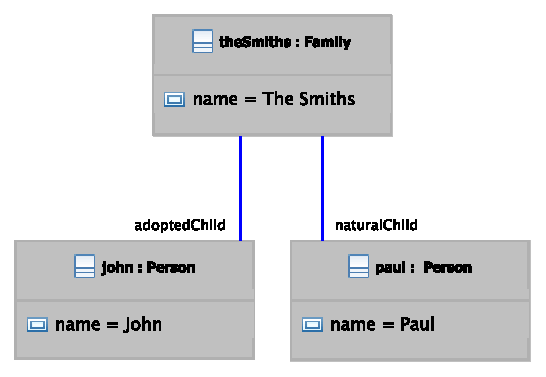
\includegraphics[height=5cm]{5.Implementation/images/successful_binding.pdf}
  \caption{Objects resulting from the binding of a conformant model}
  \label{fig:successful_binding}
\end{figure}

Metamodel-specific binding fails for non-conformant models. For example, attempting to bind the family model in Figure~\ref{fig:families_model} to the evolved families metamodel (Figure~\ref{fig:evolved_families_mm}) fails because the model uses \texttt{na\-tu\-r\-alCh\-il\-dr\-en} and \texttt{ad\-op\-t\-edCh\-il\-dr\-en} features for the type \texttt{Fa\-mi\-ly}, and these features are not defined by the evolved metamodel.

Because non-conformant models cannot be loaded, model migration must be performed by editing the underlying storage representation, which can be error-prone and tedious (Section~\ref{subsec:user-driven_co-evolution}). The sequel discusses potential solutions for loading non-conformant models.

\subsection{Potential Solutions for Loading Non-Conformant Models}
Two potential approaches to binding (and hence loading) non-conformant models have been considered and are now discussed. The benefits and drawbacks of each approach have been compared, which resulted in the selection of the second approach, binding to a metamodel-independent syntax.

\subsubsection{Store metamodel history}
Presently, modelling frameworks are used to store only the latest version of a metamodel, and hence binding fails for models that conform to a previous version of the metamodel. If modelling frameworks could access old versions of a metamodel, models that do not conform to the current version of the metamodel could be loaded by binding to a previous version of the metamodel.

\subsubsection{A metamodel-independent syntax}
Models can always be successfully bound to a \emph{metamodel-independent} representation, such as the one shown in Figure~\ref{fig:minimal_generic_metamodel}. Binding each model element results in the instantiation of a metamodel-independent type (\texttt{Ob\-je\-ct} in Figure~\ref{fig:minimal_generic_metamodel}) rather than of types defined in a specific metamodel, such as \texttt{Fa\-mi\-ly} or \texttt{Pe\-rs\-on}. Hence, binding is independent of the types defined in metamodels, and will succeed for non-conformant models.

\begin{figure}[htbp]
  \centering
  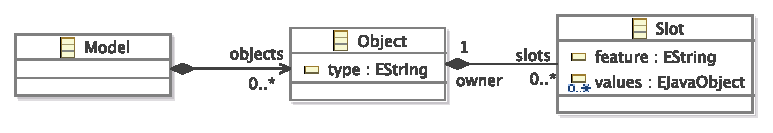
\includegraphics[width=12cm]{5.Implementation/images/slot_model_design.pdf}
  \caption[A minimal generic metamodel for MOF]{A minimal generic metamodel for MOF in Ecore, based on \cite{mof} and taken from \cite{rose09enhanced}.}
  \label{fig:minimal_generic_metamodel}
\end{figure}
   
\subsubsection{Benefits and drawbacks of the potential solutions}
The two potential solutions for loading non-conformant models have different benefits and drawbacks, which are now discussed. Storing metamodel histories would use the binding and conformance checking services provided by existing modelling frameworks, and therefore require less implementation effort than a metamodel-independent syntax, which would require bespoke binding and conformance checking services. Furthermore, structures for managing metamodel histories might be integrated with existing approaches to managing co-evolution, such as metamodel differencing approaches (Sections~\ref{subsec:inference}), for switching between different versions of a MDE workflow.

Storing metamodel histories relies on the metamodel developer to enable model migration: if the metamodel developer does not provide a metamodel that contains historical data, then binding will fail for non-conformant models. Conversely, models can be bound to a metamodel-independent syntax irrespective of the actions of the metamodel developer.

A metamodel-independent syntax has been chosen because it makes fewer assumptions of the metamodel developer, and hence facilitates user-driven as well as developer-driven co-evolution.


\subsection{Proposed Solution: A Metamodel-Independent Syntax}
\label{subsec:binding}
This section discusses the design and implementation of a metamodel-ind\-ep\-en\-de\-nt syntax, and of the binding and conformance checking services that are used to load non-conformant models. As discussed below, the metamodel-independent syntax and conformance checking service are inspired by UML \cite{uml22} and \cite{paige07metamodel}, respectively. As such, the primary contribution of this section is the implementation and integration of the syntax and services with EMF. In addition, the syntax and services have been designed to be re-usable, and hence have been used to simplify the implementation of a textual modelling notation (Section~\ref{sec:notation}) and a model migration language (Section~\ref{sec:flock}).

\subsubsection{Design}
A high-level design for the way in which the metamodel-independent syntax, binding service and conformance checking service load models is shown in Figure~\ref{fig:mmi_workflow}. The \textbf{binding service} parses XMI (the canonical storage representation of models, Section~\ref{subsec:mof}) and produces a model that conforms to the \textbf{metamodel-independent syntax}. The \textbf{conformance checking service} is used to explicitly check the conformance of a model conforming to the metamodel-independent syntax.

\begin{figure}[htbp]
	\centering
		\includegraphics*[viewport=10 590 990 760,width=11.5cm]{5.Implementation/images/mmi_workflow.pdf}
	\caption{Loading models with the metamodel-independent syntax}
	\label{fig:mmi_workflow}
\end{figure}

Binding and conformance checking were split into separate services to facilitate re-use. For example, the textual modelling notation in Section~\ref{sec:notation} re-uses the metamodel-independent syntax and conformance checking service, in conjunction with a different binding service.

\paragraph{Metamodel-independent syntax} The metamodel-independent syntax is used to represent a model without instantiating types defined by its metamodel. Its design was inspired by the metamodel for UML 2 \cite{uml212} object diagrams, which describes objects in a generic, class-independent manner. UML 2 object diagrams are specified in terms of an abstract syntax (comprising, for example, \texttt{InstanceSpecification} and \texttt{Link} classes) and a concrete syntax (comprising, for example, boxes and lines). The metamodel-independent syntax proposed here is abstract. It is not used directly by metamodel developers or users and hence a concrete syntax was not required.

Abstract syntax is typically represented as a metamodel (Section~\ref{subsec:modelling_languages}). The metamodel in Figure~\ref{fig:minimal_generic_metamodel} was used as an initial design for the metamodel-independent syntax, which contains a class for each type in the MOF metamodel that is instantiated in a model. In other words, \texttt{Ob\-je\-ct}s are used to represent each element of a model, and the \texttt{ty\-pe} attribute is used to indicate the name of the metaclass that the \texttt{Ob\-je\-ct} intends to instantiate. Similarly, \texttt{Sl\-ot}s are used to represent values in the model, and the \texttt{feature} attribute indicates the metafeature that the \texttt{Sl\-ot} intends to instantiate. The metamodel was designed to capture the information needed to perform conformance checking (described below), and implementing the conformance checking service led to a refactored metamodel, which is presented in the sequel.

COPE (Section~\ref{subsec:operator-based_co-evolution}) is also built atop a metamodel-independent syntax. However, the metamodel-independent syntaxes used by COPE and proposed here were developed independently, and both were first published in 2008 (in \cite{rose08hutn,herrmannsdoerfer08cope}).

\paragraph{Metamodel-independent binding service} The metamodel-independent binding service is a text-to-model (T2M) transformation that consumes XMI and produces a model conforming to the metamodel-independent syntax. The transformation was designed to extract all of the information pertaining to the model from XMI, translating it into the concepts defined in the metamodel-independent syntax. In particular, the binding service iterates over each tag in the XMI, and creates instances of \texttt{Ob\-je\-ct} and \texttt{Sl\-ot}. For example, when encountering a tag that represent a model element, the transformation performs the steps in Figure~\ref{fig:binding_objects}.

\begin{figure}[p]
	\begin{framed}
		\begin{enumerate}
			\item Constructs an instance of \texttt{Ob\-je\-ct}, \texttt{o}.
			\item For each attribute of the tag:
			\subitem Creates an instance of \texttt{Sl\-ot}, \texttt{s}.
			\subitem Sets \texttt{s.feature} to the name of the attribute.
			\subitem Sets \texttt{s.value} to the value of the attribute.
			\subitem Adds \texttt{s} to \texttt{o.slots}.
			\item For each child tag:
			\subitem Creates an instance of \texttt{Sl\-ot}, \texttt{s}.
			\subitem Sets \texttt{s.feature} to the name of the child tag.
			\subitem Recursively constructs an instance of \texttt{Ob\-je\-ct}, c.
			\subitem Sets \texttt{s.value} to c.
			\subitem Adds \texttt{s} to \texttt{o.slots}.
		\end{enumerate}
	\end{framed}
	\caption{Pseudo code for binding XMI tags to \texttt{Ob\-je\-ct}s.}
  \label{fig:binding_objects}
\end{figure}

\begin{figure}[p]
  \centering
  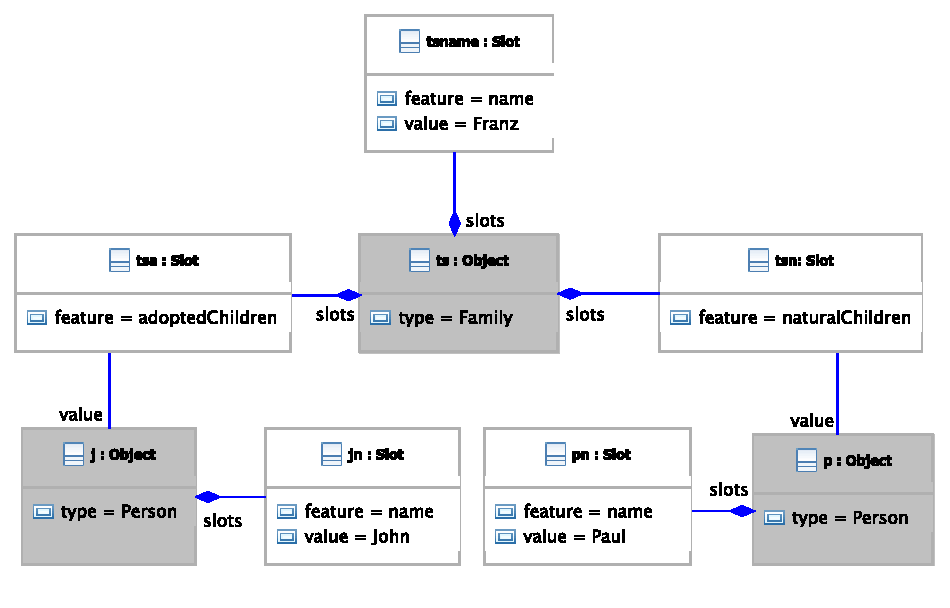
\includegraphics[width=12cm]{5.Implementation/images/generic_binding.pdf}
  \caption{Result of binding the families model with the metamodel-independent syntax}
  \label{fig:generic_binding}
\end{figure}

Applying the metamodel-independent binding service to the families model (Figure~\ref{fig:families_model}) produces three instances of \texttt{Ob\-je\-ct}, illustrated as a UML object diagram in Figure~\ref{fig:generic_binding}. For clarity, instances of \texttt{Ob\-je\-ct} are shaded, and instances of \texttt{Sl\-ot} are unshaded. The first \texttt{Ob\-je\-ct} represents the \texttt{Fa\-mi\-ly} model element and has three slots. Two of the slots are used to reference the \texttt{Pe\-rs\-on} model elements via the \texttt{na\-tu\-r\-alCh\-il\-dr\-en} and \texttt{ad\-op\-t\-edCh\-il\-dr\-en} references. 


\paragraph{Conformance checking service} Conformance is a type of inter-model consistency, between a model and its metamodel (Section~\ref{subsec:modelling_languages}), and, in MDE, inter-model consistency is often validated using a set of constraints (Section~\ref{subsubsec:model_validation}). Furthermore, \cite{paige07metamodel} demonstrates that conformance can be specified as a set of constraints between a model and its metamodel. As such, the conformance checking service has been designed as the set of constraints between models and metamodels in Figure~\ref{fig:conformance_checking_constraints}.

The conformance checking service must be interoperable with the me\-ta\-mo\-del-ind\-ep\-en\-de\-nt syntax and, hence, the constraints are specified in terms of \texttt{Ob\-je\-ct}s and \texttt{Sl\-ot}s. Clearly, to check conformance the constraints must refer to a (specific) metamodel, and the constraints are also specified in terms of concepts from the MOF metamodelling language (Section~\ref{subsec:mof}), such as \texttt{Class} and \texttt{Property}. Figure~\ref{fig:minimal_mof} shows a minimal version of the MOF metamodel.

\begin{figure}[p]
  \centering
  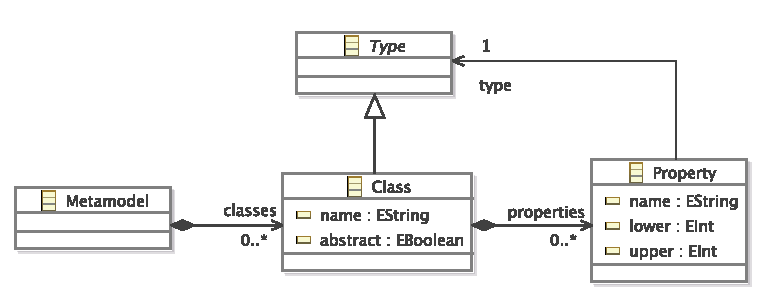
\includegraphics[width=10.5cm]{5.Implementation/images/minimal_mof.pdf}
  \caption{Minimal MOF metamodel, based on \cite{mof}.}
  \label{fig:minimal_mof}
\end{figure}

\begin{figure}[p]
	\begin{framed}
	  \begin{enumerate}
			\item Each \texttt{Ob\-je\-ct}'s \texttt{ty\-pe} must be the \texttt{na\-me} of some non-\texttt{ab\-str\-act} metamodel \texttt{Cl\-a\-ss}.
			\item Each \texttt{Ob\-je\-ct} must specify a \texttt{Sl\-ot} for each mandatory \texttt{Pr\-op\-er\-ty} of its \texttt{ty\-pe}.
			\item Each \texttt{Sl\-ot}'s \texttt{fe\-at\-u\-re} must be the name of a metamodel \texttt{Pr\-op\-er\-ty}. That \texttt{Pr\-op\-er\-ty} must belong to the \texttt{Sl\-ot}'s \texttt{ow\-n\-er}'s \texttt{ty\-pe}.
			\item Each \texttt{Sl\-ot} must be multiplicity-compatible with its \texttt{Pr\-op\-er\-ty}. More specifically, each \texttt{Sl\-ot} must contain at least as many values as its \texttt{Pr\-op\-er\-ty}'s \texttt{lo\-w\-er} bound, and at most as many values as its \texttt{Pr\-op\-er\-ty}'s \texttt{up\-p\-er} bound.
		  \item Each \texttt{Sl\-ot} must be type-compatible with its \texttt{Pr\-op\-er\-ty}. (The way in which type-compatibility is checked depends on the way in which the modelling framework is implemented).
		\end{enumerate}
	\end{framed}
  \caption{The constraints of the conformance checking service.}
  \label{fig:conformance_checking_constraints}
\end{figure}

After binding to the metamodel-independent syntax, the conformance of a model can be checked against any specific metamodel. To illustrate the value of the conformance checking service, consider again the metamodel evolution in Figure~\ref{fig:families_mms} and the bound model in Figure~\ref{fig:generic_binding}. For the evolved metamodel (Figure~\ref{fig:evolved_families_mm}), conformance checking for the model element representing the \texttt{Fa\-mi\-ly} would fail. As illustrated in Figure~\ref{fig:generic_binding}, the \texttt{Fa\-mi\-ly} \texttt{Ob\-je\-ct} defines slots for features named  \texttt{na\-tu\-r\-alCh\-il\-dr\-en} and \texttt{ad\-op\-t\-edCh\-il\-dr\-en}, which are not defined the metaclass \texttt{Fa\-mi\-ly} in Figure~\ref{fig:evolved_families_mm}. Specifically, the model element representing the \texttt{Fa\-mi\-ly} does not satisfy conformance constraint 3, which states: \emph{each \texttt{Sl\-ot}'s \texttt{fe\-at\-u\-re} must be the name of a metamodel \texttt{Pr\-op\-er\-ty}. That \texttt{Pr\-op\-er\-ty} must belong to the \texttt{Sl\-ot}'s \texttt{ow\-n\-er}'s \texttt{ty\-pe}}.

\subsubsection{Reference implementation in Java, EMF and Epsilon}
\label{subsubsec:mmi_impl}
Reference implementations of the three components were constructed with Java, EMF and Epsilon (Section~\ref{sec:mde_tools}). The way in which each component was implemented is now discussed.

\paragraph{Metamodel-independent syntax} Ecore, the metamodelling language of EMF, was used to implement the metamodel-independent syntax. The final metamodel is shown in Figure~\ref{fig:mmi_syntax_impl}, which differs slightly to the initial design (Figure~\ref{fig:minimal_generic_metamodel}). Specifically, \texttt{Sl\-ot} is abstract, has a generic type (\texttt{T}), and is the superclass of \texttt{Att\-ri\-bu\-teSl\-ot}, \texttt{Re\-fe\-re\-n\-ceSl\-ot} and \texttt{Co\-nt\-ai\-nm\-entSl\-ot}. These changes simplified the implementation of the (abstract) \texttt{ty\-peCo\-mp\-at\-ib\-i\-leWi\-th} method, which is used by the conformance checking service, and returns \texttt{true} if and only if every element of the \texttt{va\-lu\-es} attribute is type compatible with the \texttt{EC\-la\-ss\-if\-ier} parameter (a metamodel type).  

\begin{figure}[htbp]
  \centering
  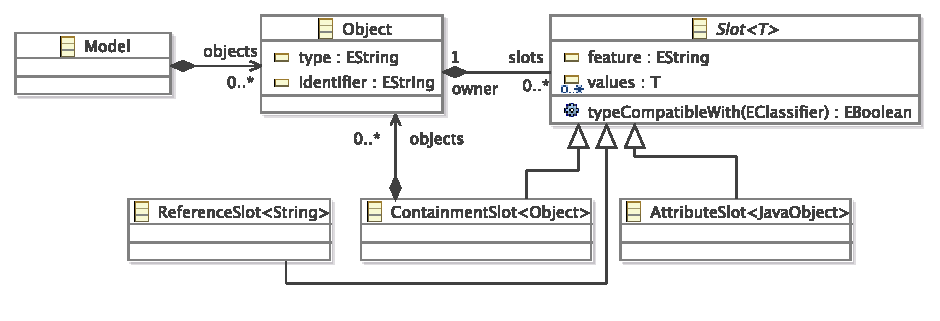
\includegraphics[width=12cm]{5.Implementation/images/slot_model_complete.pdf}
  \caption{Implemented version of the metamodel-independent syntax, in Ecore}
  \label{fig:mmi_syntax_impl}
\end{figure}

\paragraph{Binding service} A text-to-model (T2M) transformation language (Section~\ref{subsubsec:model_transformation}) could have been used to implement the binding service. However, in 2008 the Eclipse Modeling Project\footnote{\url{http://www.eclipse.org/modeling/}} did not provide a standard T2M language and using a T2M language that was not part of the Eclipse Modeling Project would have complicated installation of the service for users.

Instead, the binding service has been implemented by constructing in Java an XMI parser that emits objects conforming to the metamodel-independent syntax. Listing~\ref{lst:xmi_parser} illustrates the way in which XMI attributes are parsed. The \texttt{pr\-oc\-e\-ssAtt\-rib\-ut\-es} method is called to generate instances of \texttt{At\-tr\-ibu\-teSl\-ot} from the metamodel-independent syntax (Figure~\ref{fig:mmi_syntax_impl}). For each attribute in an XMI tag, the body of the loop is executed. If the attribute is not XMI metadata such as type information (line 4), the name and value of the attribute (lines 5 and 6) are extracted from the XMI, and used to add the value to an \texttt{At\-tr\-ibu\-teSl\-ot} with feature equal to the name of the attribute (line 8). Constructing \texttt{O\-bj\-e\-ct}s and \texttt{Sl\-ot}s is the responsibility of the \texttt{ge\-ne\-ra\-tor} object, which is an instance variable of the parser.


\begin{lstlisting}[caption=Parsing XMI attributes (in Java), label=lst:xmi_parser, language=Java]
private void processAttributes(Attributes atts) {
	for (int index = 0; index < atts.getLength(); index++) {
		
		if (!attributeIsMetadata(atts.getQName(index))) {
			final String feature = atts.getLocalName(index);
			final String value   = atts.getValue(index);
			
			generator.addAttributeValue(feature, value);
		}
	}
}
\end{lstlisting}

\paragraph{Conformance checking service} EVL (Section~\ref{subsubsec:model_validation}), a language tailored for model verification and hence suitable for rapid prototyping of consistency constraints, was used to implement the conformance constraints (Figure~\ref{fig:conformance_checking_constraints}). Listing~\ref{lst:conformance_constraint} shows the EVL constraint that checks whether each \texttt{Ob\-je\-ct}'s \texttt{ty\-pe} is a non-abstract class (constraint 1 in Figure~\ref{fig:conformance_checking_constraints}). The \texttt{ch\-e\-ck} part (line 3) verifies that a particular \texttt{Ob\-je\-ct} (referenced via the \texttt{se\-lf} keyword) refers to a metamodel type that is not abstract. If the check fails, the message (line 4) is automatically added to a set of unsatisfied constraints. The \texttt{toCl\-a\-ss} operation (lines 8-10) is used to determine the metamodel class (an instance of \texttt{EClass}) to which the \texttt{type} attribute (a \texttt{St\-ri\-ng}) of an \texttt{Ob\-je\-ct} refers. The conformance checking service returns a report of unsatisfied constraints.

Type-compatibility checks have been implemented by delegating to the type-checking methods provided by EMF. The EVL constraints call the \texttt{isTy\-peCo\-mp\-at\-ib\-leWi\-th} method on the \texttt{Sl\-ot} class. Each subclass of \texttt{Sl\-ot} provides an implementation of \texttt{isTy\-peCo\-mp\-at\-ib\-leWi\-th}, which delegates to EMF to perform type-checking.

\begin{lstlisting}[caption=A constraint (in EVL) to check that only concrete metamodel types are instantiated., label=lst:conformance_constraint, language=EVL, float=tb]
context Object {
	constraint ClassMustNotBeAbstract {
		check: not self.toClass().isAbstract()
		message: 'Cannot instantiate the abstract class: ' + self.type
	}
}

operation Object toClass() : EClass {
	return Metamodel!EClass.all.selectOne(c|c.name == self.type);
}
\end{lstlisting}

% Conformance constraints vary over modelling languages. For example, Ecore, the modelling language of EMF, is similar to but not the same as MOF. Metamodel features defined in Ecore can be marked as transient (not stored to disk) or unchangeable (read-only). Consequently in EMF, conformance constraints are required to restrict the feature value of slots to only non-transient, changeable features.

\subsection{Structures Built atop the Metamodel-Independent Syntax}
There are many potential uses for the metamodel-independent syntax described in this section. Section~\ref{sec:notation} describes a textual modelling notation integrated with the metamodel-independent syntax to achieve live conformance checking. The migration language presented in Section~\ref{sec:flock} can be used with the metamodel independent syntax to perform partial migration.

In addition to these uses, the metamodel-independent syntax is potentially useful during metamodel installation. As discussed in Section~\ref{subsec:modelling_framework_characteristics}, metamodel developers do not have access to downstream models, and conformance is implicitly enforced by modelling frameworks. Consequently, the conformance of models may be affected by the installation of a new version of a metamodel, and the conformance of models cannot be checked during installation. Typically, installing a new version of a metamodel can result in models that no longer conform to their metamodel and cannot be used with the modelling framework. Moreover, a user discovers conformance problems only when attempting to use a model after installation has completed, and not as part of the installation process.

To enable conformance checking as part of metamodel installation in EMF, the metamodel-independent syntax has been integrated with Concordance in \cite{rose10concordance}. The work was conducted outside of the scope of the thesis, and is now summarised to indicate the usefulness of the metamodel-independent syntax for supporting the automation of co-evolution activities. Concordance provides a mechanism for resolving inter-model references (such as those between models and their metamodels). Without Concordance, determining the the instances of a metamodel is possible only by checking every model in the workspace. Integrating Concordance and the metamodel-independent syntax resulted in a service, which Epsilon (Section~\ref{subsec:epsilon}) executes after the installation of a metamodel to identify the models that are affected by the metamodel changes. All models that conform to the old version of the metamodel are checked for conformance with the new metamodel. As such, conformance checking occurs automatically and immediately after metamodel installation. Conformance problems are detected and reported immediately, rather than when an affected model is next used.

\subsubsection{Summary}
Modelling frameworks implicitly enforce conformance, which presents challenges for managing co-evolution. In particular, detecting and reconciling conformance problems involves managing non-conformant models, which cannot be loaded by modelling frameworks and hence cannot be used with model editors or model management operations. The metamodel-independent syntax proposed in this section enables modelling frameworks to load non-conformant models, and has has been integrated with Concordance \cite{rose10concordance} to facilitate the reporting of conformance problems during metamodel installation. The metamodel-independent syntax, binding service and conformance checking service underpin the implementation of the textual modelling notation presented in the sequel. The benefits and drawbacks of the metamodel-independent syntax in the context of user-driven co-evolution are explored in Chapter~\ref{Evaluation}. 

%!TEX root = /Users/louis/Documents/PhD/Deliverables/Thesis/thesis.tex

\section{Textual Modelling Notation}
\label{sec:notation}
The analysis of co-evolution examples in Chapter~\ref{Analysis} highlighted two ways in which co-evolution is managed. In \emph{developer-driven} co-evolution, migration is specified by the metamodel developer in an executable format; while in \emph{user-driven co-evolution} migration is specified by the metamodel developer in prose or not at all. Performing user-driven co-evolution with modelling frameworks presents two key challenges that have not been explored by existing research. Firstly, user-driven co-evolution often involves editing the storage representation of the model, such as XMI. Model storage representations are typically not optimised for human use and hence user-driven co-evolution can be error-prone. Secondly, non-conformant model elements must be identified during user-driven co-evolution. When a multi-pass parser is used to load models, as is the case with EMF, not all conformance problems are reported at once, and user-driven co-evolution is an iterative process. In Section~\ref{sec:requirements_identification}, these challenges led to the identification of the following requirement: \emph{This thesis must demonstrate a user-driven co-evolution process that enables the editing of non-conformant models without directly manipulating the underlying storage representation and provides a sound and complete conformance report for the original model and evolved metamodel.}

Section~\ref{subsec:migration_with_xmi} illustrates some of the challenges to performing model migration with XMI, and Section~\ref{subsec:alternatives_to_xmi} discusses potential alternatives to XMI for user-driven co-evolution. Section~\ref{subsec:hutn} describes an OMG standard modelling notation that is optimised for human-usability, and Section~\ref{subsec:epsilon_hutn} presents a reference implementation of the OMG standard built atop EMF. Finally, Section~\ref{subsec:migration_with_hutn} demonstrates the wƒay in which the reference implementation of the notation has been integrated with the metamodel independent syntax described in Section~\ref{sec:mmi_syntax} to produce conformance reports. 

\subsection{Model Migration with XMI}
\label{subsec:migration_with_xmi}
The co-evolution example from Section~\ref{sec:mmi_syntax} is now used to illustrate the way in which model migration is performed by editing the underlying storage representation of a model, such as XMI (Section~\ref{subsec:mof}). Consider again the evolution of the families metamodel (Figure~\ref{fig:families_mms_repeated}) and a model conforming to the original metamodel (Figure~\ref{fig:families_model_repeated}).

\begin{figure}[htbp]
	\centering
	\subfigure[Original metamodel.]
	{
	    \label{fig:original_families_mm_repeated}
	    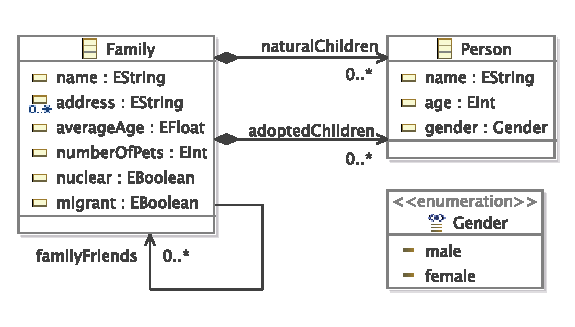
\includegraphics[scale=0.9]{5.Implementation/images/families.pdf}
	}
	\subfigure[Evolved metamodel.]
	{
	    \label{fig:evolved_families_mm_repeated}
	    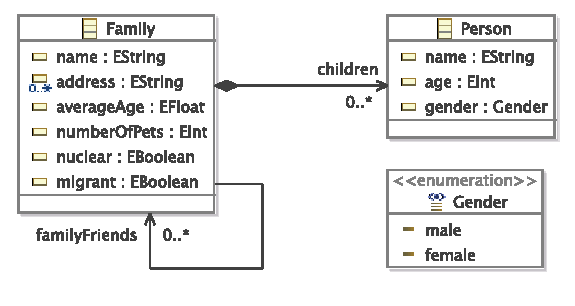
\includegraphics[scale=0.9]{5.Implementation/images/families_evolved.pdf}
	}
	\caption{Evolution of a families metamodel, based on the metamodel in \cite{hutn}.}
\label{fig:families_mms_repeated}
\end{figure}

\begin{figure}[htbp]
  \begin{center}
    \leavevmode
    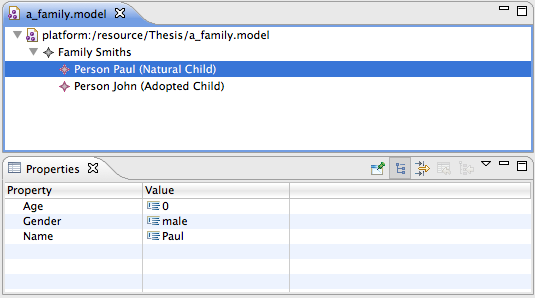
\includegraphics[width=10cm]{5.Implementation/images/family_model.png}
  \end{center}
  \caption[A family model]{A family model, which conforms to the metamodel in Figure~\ref{fig:original_families_mm_repeated}}
  \label{fig:families_model_repeated}
\end{figure}

The model in Figure~\ref{fig:families_model_repeated} does not conform to the evolved metamodel (because it uses the \texttt{na\-tu\-ralCh\-il\-dr\-en} and \texttt{ad\-op\-t\-edCh\-il\-dr\-en} features, which are not defined for \texttt{Pe\-rs\-on}), and hence cannot be loaded by the modelling framework. Migration might be achieved by editing the underlying storage representation directly (i.e. manually manipulating XMI). Listing~\ref{lst:xmi} shows the XMI for the model in Figure~\ref{fig:families_model_repeated}.

\begin{lstlisting}[caption=XMI for the family model in Figure~\ref{fig:families_model_repeated}, label=lst:xmi, language=XML]
<?xml version="1.0" encoding="ASCII"?>
<families:Family xmi:version="2.0" xmlns:xmi="http://www.omg.org/XMI" xmlns:families="families" xmi:id="_kE2LkAagEeC-FIOYrvUj0A" name="Smiths">
  <naturalChildren xmi:id="_q8RWYAagEeC-FIOYrvUj0A" name="Paul"/>
  <adoptedChildren xmi:id="_nj6TcAagEeC-FIOYrvUj0A" name="John"/>
</families:Family>
\end{lstlisting}

XMI is a concrete syntax for models, which has been optimised for use by machines and not by humans \cite{hutn}. Models often contain information that is not relevant to the domain, such as the universally unique identifiers (\texttt{xmi:id} attributes) on lines 2, 3 and 4 of Listing~\ref{lst:xmi}. Furthermore, information is often omitted to reduce the size of the model on disk. For example, the model elements on lines 3 and 4 of Listing~\ref{lst:xmi} do not specify their type (\texttt{Pe\-rs\-on}) and this is inferred from the type of the \texttt{na\-tu\-ralCh\-il\-dr\-en} and \texttt{ad\-op\-t\-edCh\-il\-dr\-en} features. Types are inferred from the metamodel by the modelling framework using a reference from the model to the metamodel. In XMI, metamodel references are expressed using XML namespaces. The XMI in Listing~\ref{lst:xmi} imports the families metamodel to a namespace (families) on line 2. The evaluation presented in Section~\ref{sec:exemplar_user-driven_co-evo} further explores the suitability of XMI for user-driven co-evolution. The remainder of this section discusses the design and implementation of a modelling notation that provides an alternative to XMI, and is tailored for human-use.

\subsection{Potential Alternatives to XMI}
\label{subsec:alternatives_to_xmi}
Two characteristics were considered when designing a notation that provides an alternative to representing models with XMI. Models can be represented textually or graphically (Section~\ref{subsec:modelling_languages}), and with a metamodel-specific or a metamodel-independent syntax (Section~\ref{sec:mmi_syntax}). The benefits and drawbacks of each option have been considered particularly with respect to their implications for user-driven co-evolution, and are now discussed.

\paragraph{Metamodel-independent vs metamodel-specific} A metamodel-specific syntax is defined in terms from the metamodel, and is often more concise than a metamodel-independent syntax. A metamodel-specific (and textual) syntax for part of the original families metamodel (Figure~\ref{fig:original_families_mm_repeated}) is shown in Listing~\ref{lst:mms_syntax}. Using the metamodel-specific syntax, the families model in Listing~\ref{lst:xmi} is represented as \texttt{Smiths:Paul(John)}. Notice that the syntax is defined in metamodel terms, such as \texttt{Fa\-mi\-ly}, \texttt{na\-tu\-ralCh\-il\-dr\-en}, and \texttt{ad\-op\-tedCh\-il\-dr\-en}. Consequently, the syntax definition can be affected by metamodel evolution, and hence cannot be used to load a model that does not conform to the metamodel. Therefore, a metamodel-specific representation is not suitable for use during user-driven co-evolution, which involves using a modelling notation with non-conformant models, and hence a metamodel-independent representation was preferred.

\begin{lstlisting}[caption=A metamodel-specific syntax for families in EBNF, label=lst:mms_syntax, language=EBNF]
family = name ":" naturalChildren "(" adoptedChildren ")"
naturalChildren = name { "," name }
adoptedChildren = name { "," name }
name = "A" | ... | "z"
\end{lstlisting}

\paragraph{Textual vs graphical} For user-driven co-evolution, the usability of the modelling notation is important because a metamodel user manipulates models with the notation to perform migration. The choice between a textual or graphical notation likely has a significant impact on usability, but it was not feasible to conduct a thorough user analysis given the time constraints of the thesis. Instead, a textual notation was selected to reduce implementation effort, and implemented to facilitate the addition of an equivalent graphical notation in future work. In particular, the concrete and abstract syntax definitions of the notation were kept separate to simplify the addition of an alternative concrete syntax in the future.

Currently, several tools exist for representing models with textual, metamodel-specific syntaxes (such as the text-to-model transformation tools discussed in Section~\ref{subsubsec:model_transformation}), but no tools exist for representing models in a metamodel-independent syntax other than XMI. \cite{steel01hutn} describe the Distributed Systems Technology Centre's TokTok project, which provided a metamodel-independent textual modelling notation, and is now inactive. The metamodel-independent representation described in \cite{muller05hutn} has been abandoned in favour of Sintaks\footnote{\url{http://www.kermeta.org/sintaks/}}, a tool for constructing metamodel-specific representations. However, the metamodel-independent representations described in \cite{steel01hutn,muller05hutn} were based on an OMG standard, Human-Usable Textual Notation (HUTN) \cite{hutn}, which defines a textual modelling notation that aims to conform to human-usability criteria \cite{hutn}. As a metamodel-independent, textual concrete syntax, HUTN was seen as an ideal starting point for designing a textual modelling notation for user-driven co-evolution. OMG HUTN is described in the sequel.

\subsection{OMG Human-Usable Textual Notation}
\label{subsec:hutn}
OMG HUTN is a textual, metamodel-independent modelling notation whose primary design goal is human-usability and ``this is achieved through consideration of the successes and failures of common programming languages'' \cite[Section 2.2]{hutn}. The HUTN specification refers to two studies of programming language usability to justify design decisions. However, the OMG specification does not evaluate the human-usability of the notation because no reference implementation exists. As HUTN is (purportedly) optimised for human-usability, using HUTN rather than XMI for user-driven co-evolution should lead to increased developer productivity. This claim is explored in Chapter~\ref{Evaluation}.

Like the metamodel presented in Section~\ref{sec:mmi_syntax}, HUTN is a metamodel-independent syntax for MOF. However, the OMG HUTN specification focuses on concrete syntax, whereas the metamodel-independent syntax presented in Section~\ref{sec:mmi_syntax} focuses on abstract syntax. In this section, the key features of HUTN are introduced, and the sequel presents a new reference implementation of HUTN. Throughout the remainder of this section, the original families metamodel (Figure~\ref{fig:original_families_mm_repeated}) is used to illustrate the notation.


\subsubsection{Basic Notation}
Listing \ref{lst:attributes} shows the construction of an \emph{object} (an instance of a metamodel class) in OMG HUTN, here an instance of the Family class from Figure \ref{fig:original_families_mm_repeated}. Line 1 specifies the metamodel \emph{package} containing the metamodel classes that can be instantiated by this model (\texttt{Fa\-mi\-lyPa\-ck\-a\-ge}). A package declaration in OMG HUTN is equivalent to a namespace import at the start of an XMI document (e.g. line 2 of Listing~\ref{lst:xmi}). In Listing~\ref{lst:attributes}, line 2 names the metamodel class to be instantiated (\texttt{Fa\-mi\-ly}) and gives an identifier for the object (\texttt{The Sm\-it\-hs}). Lines 3 to 7 define \emph{attribute values}; in each case, the data value is assigned to the attribute with the specified name. The encoding of the value depends on its type: strings are delimited by any form of quotation mark; multi-valued attributes use comma separators, etc.

The metamodel in Figure \ref{fig:original_families_mm_repeated} has a \emph{simple reference} (\texttt{fa\-mi\-lyFr\-ie\-n\-ds}) and two \emph{containment references} (\texttt{ad\-op\-t\-edCh\-il\-dr\-en}; \texttt{na\-tu\-r\-alCh\-il\-dr\-en}). The OMG HUTN representation embeds a contained object directly in the parent object, as shown in Listing \ref{lst:containment}. A simple reference can be specified using the type and identifier of the referred object, as shown in Listing \ref{lst:non-contained}. Like attribute values, both styles of reference are preceded by the name of the meta-feature.

\begin{lstlisting}[caption={[Specifying attributes with HUTN]Specifying attributes with HUTN, taken from \cite{rose08hutn}}, label=lst:attributes, language=HutnFamilies]
FamilyPackage "families" {
    Family "The Smiths" {
        nuclear: true
        name: "The Smiths"
        averageAge: 25.7
        numberOfPets: 2
        address: "120 Main Street", "37 University Road"
    }
}
\end{lstlisting}

\begin{lstlisting}[caption={[Specifying a containment reference with HUTN]Specifying a containment reference with HUTN, taken from \cite{rose08hutn}}, label=lst:containment, language=HutnFamilies]
FamilyPackage "families" {
    Family "The Smiths" {
        naturalChildren: Person "John" { name: "John" },
                                Person "Jo" { gender: female }
    }
}
\end{lstlisting}


\begin{lstlisting}[caption={[Specifying a simple reference with HUTN]Specifying a simple reference with HUTN, taken from \cite{rose08hutn}}, label=lst:non-contained, language=HutnFamilies]
FamilyPackage "families" {
    Family "The Smiths" {
        familyFriends: Family "The Does"
    }
    Family "The Does" {}
}
\end{lstlisting}


\subsubsection{Keywords and Adjectives}
In general, a metamodel-independent syntax (such as OMG HUTN) will not be as concise as a metamodel-specific concrete syntax. However, OMG HUTN does define optional syntactic shortcuts to make model specifications more compact. The OMG HUTN specification aims to make the syntactic shortcuts intuitive \cite[pg2-4]{hutn}.

Two of the syntactic shortcuts relate to Boolean-valued attributes and are now discussed; a complete list of syntactic shortcuts is given in \cite{hutn}. OMG HUTN permits the use of an attribute name to represent the value \texttt{true}, or the attribute name prefixed with a tilde to represent the value \texttt{false}). When used in the body of the object, this style of Boolean-valued attribute represents a \emph{keyword}. A keyword used to prefix an object declaration is called an \emph{adjective}. Listing \ref{lst:boolean} shows the use of both an attribute keyword (\texttt{\textasciitilde nuclear} on line 6) and adjective (\texttt{\textasciitilde migrant} on line 2), and states that \texttt{The Sm\-it\-hs} are \texttt{mi\-gr\-a\-nt} and that \texttt{The Do\-es} are not \texttt{nu\-cl\-e\-ar}.

\begin{lstlisting}[caption={[Using keywords and adjectives in HUTN]Using keywords and adjectives in HUTN, taken from \cite{rose08hutn}}, label=lst:boolean, language=HutnFamilies]
FamilyPackage "families" {
    migrant Family "The Smiths" {}

    Family "The Does" {
        averageAge: 20.1
        ~nuclear
        name: "The Does"
    }
}
\end{lstlisting}


% \subsubsection{Inter-Package References}
% \label{subsubsec:inter-package_references}
% To conclude the summary of the notation, two advanced features defined in the HUTN specification are discussed. The first enables objects to refer to other objects in a different package, while the second provides means for specifying the values of a reference for all objects in a single construct (which can be used, in some cases, to simplify the specification of complicated relationships).
% 
% \begin{lstlisting}[caption=Referencing objects in other packages with HUTN., label=lst:fullyqualified, language=HutnFamilies]
% FamilyPackage "families" {
%     Family "The Smiths" {}
% }
% VehiclePackage "vehicles" {
%     Vehicle "The Smiths' Car" {
%         owner: FamilyPackage.Family "families"."The Smiths"
%     }
% }
% \end{lstlisting}
% 
% To reference objects between separate package instances in the same document, the package identifier is used to construct a fully-qualified name. Suppose a second package is introduced to the metamodel in Figure \ref{fig:example-mm}. Among other concepts, this package introduces a Vehicle class, which defines an owner reference of type Family. Listing \ref{lst:fullyqualified} illustrates the way in which the owner feature can be populated. Note that the fully-qualified form of the class utilises the names of elements of the metamodel, while the fully-qualified form of the object utilises only HUTN identifiers defined in the current document.
% 
% The HUTN specification defines name scope optimisation rules, which allow the definition above to be simplified to: \texttt{owner: Family "The Smiths"}, assuming that the VehiclePackage does not define a Family class, and that the identifier ``The Smiths'' is not used in the VehiclePackage block.


\subsubsection{Alternative Reference Syntax}
In addition to the syntax defined in Listings \ref{lst:containment} and \ref{lst:non-contained}, OMG HUTN defines two alternative syntactic constructs for specifying the value of references. For example, Listing \ref{lst:assocblock} demonstrates the use of a reference block for defining \texttt{The Does} as friends with both \texttt{The Smiths} and \texttt{The Bloggs}.

\begin{lstlisting}[caption={[Using a reference block in HUTN]Using a reference block in HUTN, taken from \cite{rose08hutn}}, label=lst:assocblock, language=HutnFamilies]
FamilyPackage "families" {
    Family "The Smiths" {}
    Family "The Does" {}
    Family "The Bloggs" {}
    
    familyFriends {
        "The Does" "The Smiths"
        "The Does" "The Bloggs"
    }
}
\end{lstlisting}

Listing \ref{lst:associnfix} illustrates a further alternative syntax for references, which employs an infix notation. 

\begin{lstlisting}[caption={[Using an infix reference in HUTN]Using an infix reference in HUTN, taken from \cite{rose08hutn}}, label=lst:associnfix, language=HutnFamilies]
FamilyPackage "families" {
    Family "The Smiths" {}
    Family "The Does" {}
    Family "The Bloggs" {}
    
    Family "The Smiths" familyFriends Family "The Does";
    Family "The Smiths" familyFriends Family "The Bloggs";
}
\end{lstlisting}

The reference block (Listing~\ref{lst:assocblock}) and infix (Listing~\ref{lst:associnfix}) notations are syntactic variations on -- and have identical semantics to -- the reference notation shown in Listings \ref{lst:containment} and \ref{lst:non-contained}.


\subsubsection{Customisation via Configuration}
The OMG HUTN specification allows some limited, metamodel-specific customisation of the notation, using \emph{configuration rules}. Customisations include a parametric form of object instantiation; renaming of metamodel elements; specifying the default value of a feature; and providing a default identifier for classes of object.


\subsection{Reference Implementation: Epsilon HUTN}
\label{subsec:epsilon_hutn}
To investigate the extent to which OMG HUTN can be used for user-driven co-evolution, a reference implementation, Epsilon HUTN, has been designed and implemented. This section describes the way in which Epsilon HUTN was implemented using a combination of model-management operations. From text conforming to the OMG HUTN syntax (described above), Epsilon HUTN produces an equivalent model that can be managed with EMF (Section~\ref{subsec:emf}). The sequel demonstrates the way in which Epsilon HUTN can be used for user-driven co-evolution.

\subsubsection{Design of Epsilon HUTN}
Implementing OMG HUTN involved building a tool for producing an EMF model (i.e. a model represented in XMI) from text conforming to the OMG HUTN syntax (described above). Essentially then, Epsilon HUTN can be regarded as a parser (that emits models), or as a text-to-model transformation. Several approaches to constructing Epsilon HUTN were considering, including: using a text-to-model (T2M) transformation tool (Section~\ref{subsubsec:model_transformation}), using a domain-specific language (DSL) framework (Section~\ref{subsec:dsls}), and using MDE tools and techniques such as EMF (Section~\ref{subsec:emf}), Epsilon (Section~\ref{subsec:epsilon}) and metamodelling.

As was the case for the design and implementation of the metamodel-independent syntax (Section~\ref{sec:mmi_syntax}), the author preferred to avoid dependencies on tools that were not part of the Eclipse Modelling Project (in order not to complicate installation of the notation for users). In 2008, the Eclipse Modeling Project\footnote{\url{http://www.eclipse.org/modeling/}} did not provide a standard T2M language or DSL framework, and so these implementation strategies were discounted.

Instead, Epsilon HUTN was constructed using existing languages of the Epsilon platform. To parse HUTN source, a parser was generated with the ANTLR parser generator tool \cite{parr07antlr}, which had been used successfully to implement parsers for the other task-specific languages of Epsilon. A parser generated with ANTLR emits an abstract syntax tree (a set of Java objects that conform to a simple tree data structure), from which the Epsilon HUTN tool needs to produce an EMF model.

\begin{figure}[htbp]
  \centering
  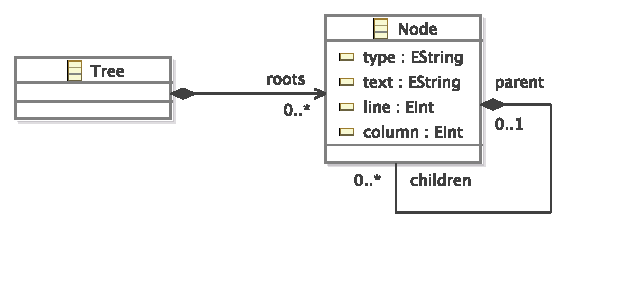
\includegraphics[width=8cm]{5.Implementation/images/ast_metamodel.pdf}
  \caption{A metamodel for abstract syntax trees, in Ecore}
  \label{fig:ast_metamodel}
\end{figure}

The abstract syntax tree produced by ANTLR can be regarded as a model (conforming to the metamodel in Figure~\ref{fig:ast_metamodel}) and hence, producing an EMF model from the abstract syntax tree can be regarded as a model-to-model transformation. Epsilon HUTN, however, was designed as two separate model-to-model transformations, for two reasons. Firstly, initial prototyping highlighted that the difference between a model represented in terms of the tree metamodel in Figure~\ref{fig:ast_metamodel} and the same model represented in metamodel-specific terms is vast, and the logic required to perform a one-step transformation quickly became complicated even for simple models. In particular, each transformation rule would have required a lengthly guard statement, which would have been difficult to debug and maintain. Secondly, it became apparent that the concrete syntax defined in OMG HUTN could be transformed to the metamodel-independent syntax defined in Section~\ref{sec:mmi_syntax}, which would reduce implementation effort by re-using the metamodel and conformance checking service described in Section~\ref{sec:mmi_syntax}.

\subsubsection{Implementation of Epsilon HUTN}
For the reasons outlined above, Epsilon HUTN is implemented using two model-to-model transformations. Figure \ref{fig:architecture} outlines the workflow through Epsilon HUTN, from HUTN source text to an EMF instantiation of the target model. The HUTN model specification is parsed to an abstract syntax tree using a HUTN parser specified in ANTLR \cite{parr07antlr}. From this, a Java postprocessor is used to construct an instance of the simple AST metamodel in Figure~\ref{fig:ast_metamodel}. Using ETL, a M2M transformation is applied to produce an intermediate model, which is an instance of the metamodel-independent syntax discussed in Section~\ref{sec:mmi_syntax}. Validation is performed on the intermediate model to ensure that the syntactic constraints specified in the OMG HUTN specification are satisfied\footnote{For example, no two objects may have the same identifier.}, and that the model conforms to the target metamodel. Conformance checking is achieved by re-using the service presented in Section~\ref{sec:mmi_syntax}. Finally, a M2T transformation on the target metamodel, specified in EGL, produces a further M2M transformation, which consumes the intermediate model and produces the target model\footnote{This final step involves a higher-order transformation (a M2T transformation is used to produce a M2M transformation), and is described in more detail below.}.

\begin{figure}[htbp]
  \begin{center}
    \leavevmode
    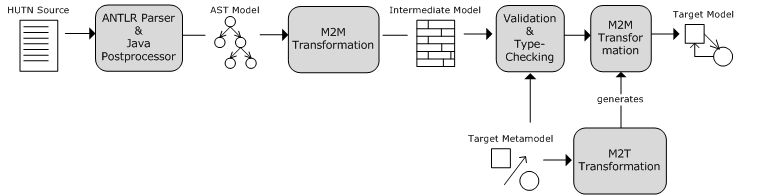
\includegraphics[scale=0.44]{5.Implementation/hutn_workflow.png}
  \end{center}
  \caption{The architecture of Epsilon HUTN.}
  \label{fig:architecture}
\end{figure}

The modular architecture in Figure~\ref{fig:architecture} facilitates the re-use of the metamodel-independent syntax and conformance checking service described in Section~\ref{sec:mmi_syntax}, and hence reduced implementation effort. A small modification was made to the metamodel-independent syntax to facilitate the implementation of Epsilon HUTN: an additional metaclass, \texttt{Pa\-ck\-a\-geOb\-je\-ct}, was added to the metamodel-independent syntax. In OMG HUTN, packages are used to segregate a model such that different parts of a OMG HUTN document can refer to different metamodels. Consequently, a \texttt{Pa\-ck\-a\-geOb\-je\-ct} has a type (i.e. the metamodel to which its contents refer), an optional identifier (used for inter-package references) and contains any number of \texttt{Ob\-je\-ct}s. To avoid confusion with \texttt{Pa\-ck\-a\-geOb\-je\-ct}, the \texttt{Ob\-je\-ct} class in the metamodel-independent syntax was renamed to \texttt{Cl\-a\-ssOb\-je\-ct}. The version of the metamodel-independent syntax used with Epsilon HUTN is shown in Figure~\ref{fig:mmi_syntax_hutn}.

\begin{figure}[htbp]
  \centering
  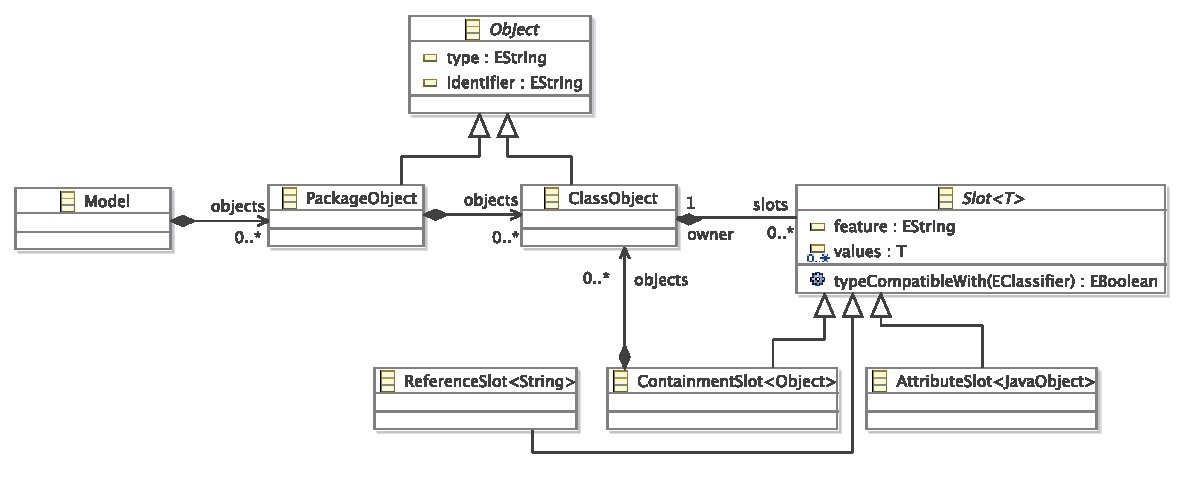
\includegraphics[width=12cm]{5.Implementation/images/slot_model_final.pdf}
  \caption{Final version of the metamodel-independent syntax, in Ecore}
  \label{fig:mmi_syntax_hutn}
\end{figure}

Each phase of the architecture in Figure~\ref{fig:architecture} is now discussed in detail. Note that, in this section, instances of the metamodel-independent syntax producing during the execution of the HUTN workflow are termed an \textit{intermediate model}.

\paragraph{Parsing the HUTN Source}
A parser for OMG HUTN was constructed using ANTLR \cite{parr07antlr}, a parser generator tool. ANTLR produces a parser from an annotated EBNF grammar definition. Part of the grammar definition used by Epsilon HUTN is shown in Listing~\ref{lst:hutn_grammar} and is used to generate parser rules that process the body of \texttt{Cl\-a\-ssOb\-je\-ct}s. The \texttt{attr} rule on line 4, for example, matches any number of comma separated attribute values or the \texttt{null} keyword.

Epsilon HUTN uses a simple, bespoke Java post-processor to construct instances of the abstract syntax tree metamodel (Figure~\ref{fig:ast_metamodel}) from the Java objects produced by ANTLR. Specifically, the post-processor copies the Java objects produced by the parser into an EMF resource, and hence produces a model that can be managed with EMF.

\begin{lstlisting}[caption=An extract of the Epsilon HUTN grammar definition in EBNF, label=lst:hutn_grammar, language=EBNF]
cls_contents = feature | adjective
feature = NAME ASSIGNMENT feature_contents
feature_contents = attr | refs | containments
attr = attr_value { COMMA attr_value } | NULL
\end{lstlisting}

\paragraph{AST Model to Intermediate Model}
Epsilon HUTN uses ETL \cite{kolovos08etl} for specifying M2M transformation. One of the transformation rules from Epsilon HUTN is shown in Listing \ref{lst:m2m}. The rule transforms a \texttt{No\-de} with type \texttt{na\-me} (which could represent a \texttt{P\-ac\-ka\-geOb\-je\-ct} or a \texttt{Cl\-a\-ssOb\-je\-ct}) to a \texttt{P\-ac\-ka\-geOb\-je\-ct} in the intermediate model. The guard (line 5) specifies that a name node will only be transformed to a \texttt{P\-ac\-ka\-geOb\-je\-ct} if the node has no parent (i.e. it is a top-level node, and hence a package rather than a class). The body of the rule states that the type, line number and column number of the package are determined from the text, line and column attributes of the \texttt{No\-de} object. On line 11, a \texttt{Co\-nt\-ai\-nm\-e\-ntSl\-ot} is instantiated to hold the children of this \texttt{P\-ac\-ka\-geOb\-je\-ct}. The children of the \texttt{No\-de} object are transformed to the intermediate model (using a method built into ETL, \texttt{eq\-ui\-va\-lent()}), and added to the \texttt{Co\-nt\-ai\-nm\-e\-ntSl\-ot}.

\begin{lstlisting}[caption=Transforming Nodes to PackageObjects with ETL., label=lst:m2m, language=ETL]
rule NameNode2PackageObject
    transform n : AntlrAst!Node
    to p : Intermediate!PackageObject {

    guard : n.type == 'Name' and n.parent.isUndefined()

    p.type := n.text;
    p.line := n.line;
    p.col  := n.column;

    var slot := new Intermediate!ContainmentSlot;
    for (child in n.children) {
        slot.objects.add(child.equivalent());
    }
    if (slot.objects.notEmpty()) {
        p.slots.add(slot);
    }
}
\end{lstlisting}

\paragraph{Intermediate Model Validation}
An advantage of the two-stage transformation is that contextual analysis can be specified in an abstract manner -- that is, without having to express the traversal of the AST. This gives clarity and minimises the amount of code required to define syntatic constraints.

\begin{lstlisting}[caption=A constraint (in EVL) to check that all identifiers are unique., label=lst:constraint, language=EVL]
context ClassObject {
    constraint IdentifiersMustBeUnique {
        guard: self.id.isDefined()
        check: ClassObject.all
                   .select(c|c.id = self.id).size() = 1;
        message: `Duplicate identifier: ' + self.id
    }
}
\end{lstlisting}

Epsilon HUTN uses EVL \cite{kolovos08evl} to specify validation, resulting in highly expressive syntactic constraints. An EVL constraint comprises a guard, the logic that specifies the constraint, and a message to be displayed if the constraint is not met. For example, Listing \ref{lst:constraint} specifies the constraint that every HUTN class object has a unique identifier.

In addition to the syntactic constraints defined in the OMG HUTN specification, the EVL constraints for checking conformance (Section~\ref{sec:mmi_syntax}) are also executed on the model at this stage.

\paragraph{Intermediate Model to Target Model}
When the intermediate model conforms to the target metamodel, the intermediate model can be transformed to an instance of the target metamodel. In other words, the model can be represented in a metamodel-specific manner and, for example, saved to disk using XMI. In generating the target model from the intermediate model (Figure \ref{fig:architecture}), the transformation uses information from the target metamodel, such as the names of classes and features. A typical approach to this category of problem is to use a higher-order transformation (HOT) on the target metamodel to generate the desired transformation \cite{tisi09hot}. Currently, ETL cannot be used to produce a transformation from a transformation and hence Epsilon HUTN uses a slightly different approach: the transformation to the target model is produced by executing a M2T transformation on the target metamodel, using EGL \cite{rose08egl}. EGL is a template-based M2T language; \verb|[% %]| tag pairs are used to denote dynamic sections, which may produce text when executed; any code not enclosed in a \verb|[% %]| tag pair is included verbatim in the generated text.

Listing \ref{lst:generate} shows part of the M2T transformation used by Epsilon HUTN. When executed on the target metamodel, the M2T transformation generates an ETL program (i.e. a M2M transformation). The generated ETL code transforms an intermediate model to a model that conforms to the target metamodel. The loop beginning on line 1 iterates over each metaclass in the target metamodel, producing a M2M transformation rule. The generated transformation rule consumes a \texttt{Cl\-a\-ssOb\-je\-ct} in the intermediate model and produces an element of the target model. The guard of the generated transformation rule (line 6) ensures that only \texttt{Cl\-a\-ssOb\-je\-ct} with a type equal to the current meta-class are transformed by the generated rule. To generate the body of the rule, the M2T transformation iterates over each structural feature of the current meta-class, and generates appropriate transformation code for populating the values of each structural feature from the slots on the class object in the intermediate model. The part of the M2T transformation that generates the body of M2M transformation rule is omitted in Listing~\ref{lst:generate} because it contains a large amount of code for interacting with EMF, which is not relevant to this discussion.

\begin{lstlisting}[caption={[Higher-order transformation with EGL]Part of the M2T transformation (in EGL) that takes a target metamodel and generates an intermediate model to target model transformation (in ETL).}, label=lst:generate, language=EGL]
[% for (class in EClass.allInstances()) { %]
rule Object2[%=class.name%]
  transform o : Intermediate!ClassObject
  to t : Model![%=class.name%] {

    guard: o.type = `[%=class.name%]'

    -- body omitted
  }
[% } %]
\end{lstlisting}

To illustrate the way in which Epsilon HUTN generates a target model from an intermediate model, the M2T transformation in Listing~\ref{lst:generate} is applied to the the families metamodel in Figure~\ref{fig:original_families_mm_repeated}. The M2T transformation generates the two M2M transformation rules in Listing~\ref{lst:hutn_generated_transformation}. The rules produce instances of \texttt{Fa\-mi\-ly} and \texttt{Pe\-rs\-on} from instances of \texttt{Cl\-a\-ssOb\-je\-ct} in the intermediate model. The body of each rule copies the values from the slots of the \texttt{Cl\-as\-sOb\-je\-ct} to the \texttt{Fa\-mi\-ly} or \texttt{Pe\-rs\-on} in the target model. Lines 7-9, for example, copy the value of the name \texttt{Sl\-ot} (if one is specified) to the target \texttt{Fa\-mi\-ly}.

\begin{lstlisting}[caption=The M2M transformation generated for the Families metamodel, label=lst:hutn_generated_transformation, language=ETL]
rule Object2Family
  transform o : Intermediate!ClassObject
  to t : Model!Family {

    guard: o.type = 'Family'

    if (o.hasSlot('name')) {
			t.name := o.findSlot('name').values.first;
		}
		
		if (o.hasSlot('address')) {
			for (value in o.findSlot('address').values) {
				t.address.add(value);
			}
		}
		
		-- remainder of body omitted
  }

rule Object2Person
  transform o : Intermediate!ClassObject
  to t : Model!Person {

    guard: o.type = 'Person'

    if (o.hasSlot('name')) {
			t.name := o.findSlot('name').values.first;
		}
		
		-- remainder of body omitted
  }
\end{lstlisting}

Currently, Epsilon HUTN can be used only to generate EMF models. Support for other modelling languages would require different transformations between intermediate and target model. In other words, for each target modelling language, a new EGL template would be required. The transformation from AST to intermediate model is independent of the target modelling language and would not need to change. As EMF is arguably the most widely-used modelling framework today, support for other modelling frameworks is not crucial for exploring the suitability of HUTN for user-driven co-evolution. However, one interesting example of metamodel evolution predates EMF: the changes made to UML between versions 1.5 and 2.0 of the specification. Because the UML 1 specifications use a version of MOF that is not supported by EMF, the current version of Epsilon HUTN cannot be used for migrating UML 1 models. Several other examples, however, were available for evaluating Epsilon HUTN, and so support for other modelling frameworks was not crucial in the context of the thesis research.

\subsubsection{Compliance to OMG HUTN}
Epsilon HUTN is a reference implementation of the OMG HUTN standard. There are, however, a few differences between the implementation in Epsilon and the OMG standard. The differences are now discussed and justified. The discussion is based on\footnote{\url{http://www.eclipse.org/gmt/epsilon/doc/articles/hutn-compliance/}}, which provides an up-to-date report of Epsilon HUTN's compliance to the OMG HUTN standard.

\begin{table}
	\centering
	\begin{tabular}{|c|c|c|}
		\hline
		\textbf{OMG HUTN} & \multicolumn{2}{|c|}{\textbf{Epsilon HUTN}} \\
		\hline
		\textbf{Feature} & \textbf{Supported?}          & \textbf{Details of support} \\
		\hline
		\hline
		Packages                                    & Yes                       & \\
		\hline                                                                    
		\multirow{3}{*}{Classes}                    & \multirow{3}{*}{Partial}  & Not yet supported:      \\
		                                            &                           & parametric attributes,  \\
		                                            &                           & enumeration adjectives. \\
		\hline                                                                    
		\multirow{2}{*}{Attributes}                 & \multirow{2}{*}{Yes}      & Corrects a mistake \\
		                                            &                           & in the standard. \\
		\hline                                                                    
		References                                  & Yes                       & \\
		\hline                                                                                   
		Classifier-level attributes                 & Yes                       & \\
		\hline                                                                                   
		Data values                                 & Yes                       & \\
		\hline                                                     
		\multirow{2}{*}{Inline configuration (6.9)} & \multirow{2}{*}{No}       & A configuration model \\
		                                            &                           & is used instead. \\
		\hline
		\multirow{3}{*}{Configuration rules (5)}    & \multirow{3}{*}{Partial}  & Not yet supported:      \\
		                                            &                           & parametric attributes,  \\
		                                            &                           & enumeration adjectives. \\
		\hline
	\end{tabular}
	\label{tab:hutn}
	\caption{Compliance of Epsilon HUTN to OMG HUTN}
\end{table}

Table~\ref{tab:hutn} summarises the differences between Epsilon HUTN and the OMG HUTN standard. Epsilon HUTN does not support two of the syntactic shortcuts described for classes in the OMG HUTN standard: parametric attributes and enumeration adjectives. The former are used to specify attribute values in a parametric form (e.g. \texttt{Point (0,0)}, for creating a \texttt{Po\-i\-nt} object with \texttt{x} and \texttt{y} attributes with value 0). The latter allows an enumeration value to prefix an object definition (e.g. \texttt{female Person} for creating a \texttt{Pe\-rs\-on} with \texttt{fe\-ma\-le} gender). The attribute to which the parametric or enumeration values are bound is specified using OMG HUTN configuration rules (Section~\ref{subsec:hutn}). Parametric attribute and enumeration adjectives were not implemented to reduce the amount of time required to build Epsilon HUTN. Alternative (albeit less concise) notion can be used to express models without using parametric attribute and enumeration adjectives.

Section 6.4 of the OMG HUTN standard \cite{hutn} appears to contain a mistake in the grammar definition. Grammar rule 20 implies that an attribute's name is optional when specifying a keyword attribute, and that an empty string or a tilde character are valid forms of a keyword attribute. However, the prose describing grammar rule 20 proposes no semantics for an empty string or a tilde character as a keyword attribute. Consequently, Epsilon HUTN deviates from grammar rule 20 of the OMG HUTN standard, and requires an attribute name for every keyword attribute.

Finally, the OMG HUTN standard defines syntax for specifying configuration rules \emph{inline}, at the start of a HUTN document. Epsilon HUTN does not support inline configuration, and Epsilon HUTN documents are configured with a configuration model, which is constructed using an EMF model editor. Using a configuration model rather than inline configuration reduced the time required to implement Epsilon HUTN and facilitated re-use of configuration models between HUTN documents.

The OMG HUTN standard does not include a set of compliance tests for reference implementations. Instead, the compliance of Epsilon HUTN to OMG HUTN was checked using the many examples of HUTN documents in the OMG HUTN standard \cite{hutn}. The examples were used to create a suite of executable compliance test cases, which were run frequently during the development of Epsilon HUTN.
 

\subsection{Migration with Epsilon HUTN}
\label{subsec:migration_with_hutn}
Used in combination with the metamodel-independent syntax presented in Section~\ref{sec:mmi_syntax}, Epsilon HUTN facilitates user-driven co-evolution using the workflow in Section~\ref{fig:hutn_process_implementation}, which provides an alternative to the user-driven co-evolution workflow observed in Section~\ref{subsec:user-driven_co-evolution}. First, the user attempts to load a model in the model editor\footnote{The workflow in Figure~\ref{fig:hutn_process_implementation} assumes a graphical model editor, such as those generated by GMF, but any editor built atop EMF will exhibit the same behaviour.}. If the model is non-conformant and cannot be loaded, the user clicks a ``Generate HUTN'' menu item provided by Epsilon HUTN. Epsilon HUTN then binds the model to the metamodel-independent syntax and unparses the bound model to produce HUTN source code equivalent to XMI representation of the non-conformant model.

To support the final step of the workflow in Figure~\ref{fig:hutn_process_implementation}, Epsilon HUTN provides an editor for HUTN documents that is integrated with the conformance checking service described in Section~\ref{sec:mmi_syntax}. The user edits the HUTN document to reconcile conformance problems (i.e. perform migration), and Epsilon HUTN automatically performs conformance checking as the user edits the HUTN document. When the conformance problems are fixed, the user saves the HUTN document and Epsilon HUTN automatically generates XMI for the conformant model (using the model transformations described in Section~\ref{subsec:epsilon_hutn}). The conformant model can then be loaded in the model editor.

\begin{figure}[htbp]
	\centering
	\includegraphics*[viewport=80 290 760 550,height=4.75cm]{6.Evaluation/images/user_driven/hutn_process.pdf}
	\caption{User-driven co-evolution with dedicated structures}
	\label{fig:hutn_process_implementation}
\end{figure}

To demonstrate the way in which HUTN can be used to perform migration, the XMI shown in Listing~\ref{lst:xmi} is represented using OMG HUTN in Listing~\ref{lst:non-conformant_hutn}. Recall that the XMI describes a \texttt{Fa\-mi\-ly} with one adopted and one natural child.

\begin{lstlisting}[caption=OMG HUTN for people with mothers and fathers., label=lst:non-conformant_hutn, language=HutnFamilies]
FamilyPackage "families" {
    Family "Smiths" {
	      name: "Smiths"
	      naturalChildren: Person { name: "Paul" }
		    adoptedChildren: Person { name: "John" }
		}
}
\end{lstlisting}

If the Families metamodel now evolves such that children are modelled using one rather than two features (Figure~\ref{fig:evolved_families_mm_repeated}), Epsilon HUTN reports conformance problems on the HUTN document using the conformance checking service described in Section~\ref{sec:mmi_syntax}, as illustrated by the screenshot in Figure~\ref{fig:hutn_conformance_reporting}.

\begin{figure}[htbp]
  \begin{center}
    \leavevmode
    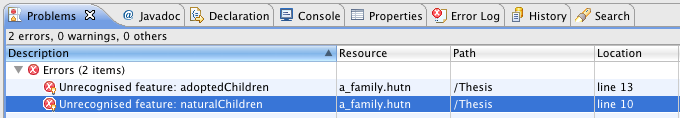
\includegraphics[scale=0.44]{5.Implementation/hutn_conformance_reporting.png}
  \end{center}
  \caption{Conformance problem reporting in Epsilon HUTN.}
  \label{fig:hutn_conformance_reporting}
\end{figure}

Resolving the conformance problems requires the user to merge the values for \texttt{ad\-op\-t\-edCh\-il\-dr\-en} and \texttt{na\-tu\-ralCh\-il\-dr\-en} into a set of values for the new feature, \texttt{ch\-il\-dr\-en}. The Epsilon HUTN development tools provide content assistance, which might be useful in this situation. Listing~\ref{lst:conformant_hutn} shows a HUTN document that conforms to the evolved metamodel in which adopted and natural children are specified using a single feature, \texttt{ch\-il\-dr\-en}.

\begin{lstlisting}[caption=HUTN for people with parents., label=lst:conformant_hutn, language=HutnFamilies]
FamilyPackage "families" {
    Family "Smiths" {
	      name: "Smiths"
	      children: Person { name: "Paul" },
                  Person { name: "John" }
		}
}
\end{lstlisting}

When the user saves the reconciled HUTN document, Epsilon HUTN will automatically generate XMI for the (now) conformant model, and migration is complete. Compared to the user-driven co-evolution workflow observed in Section~\ref{subsec:user-driven_co-evolution}, the workflow presented in Figure~\ref{fig:hutn_process_implementation} provides live conformance checking and a modelling notation that is optimised for humans rather than for machines. The two workflows are compared and evaluated in Chapter~\ref{Evaluation}.

\subsection{Summary}
In this section, a textual modelling notation for performing model migration has been designed and implemented. The notation proposed in this section is based on the OMG HUTN standard, which was described in Section~\ref{subsec:hutn}. The design and implementation of Epsilon HUTN, an implementation of OMG HUTN for EMF, was discussed in this section. Integration of Epsilon HUTN with the metamodel-independent syntax in Section~\ref{sec:mmi_syntax} facilitates user-driven co-evolution with a textual modelling notation other than XMI, as demonstrated by the example above. The user-driven co-evolution workflow presented in Section~\ref{subsec:migration_with_hutn} is evaluated in Chapter~\ref{Evaluation}. The remainder of this chapter focuses on developer-driven co-evolution, in which model migration strategies are executable.
%!TEX root = /Users/louis/Documents/PhD/Deliverables/Thesis/thesis.tex

\section[An Analysis of Languages used for Model Migration][An Analysis of Model Migration Languages]{An Analysis of Languages used for Model Migration}
\label{sec:analyis_of_languages_used_for_migration}
In contrast to the previous section, this section focuses on \emph{developer-driven} co-evolution, in which migration is specified as a program that metamodel users execute to migrate their models. Section~\ref{subsec:co-evolution_categorisation} discussed existing approaches to model migration, highlighting variation in the languages used for specifying migration strategies. In this section, the results of comparing migration strategy languages are described, using a new example of metamodel evolution (Section~\ref{subsec:co-evo_example}). From the comparison, requirements for a domain-specific language for specifying and executing model migration strategies are derived (Section~\ref{subsec:analysis}). The sequel describes an implementation of a model migration language based on the analysis presented here. The work described in this section has been published in \cite{rose10flock}.

\subsection{Co-Evolution Example}
\label{subsec:co-evo_example}
This section uses the Petri net metamodel evolution to compare model migration languages. The example is often used in co-evolution literature, for example \cite{cicchetti08automating,garces09managing,wachsmuth07metamodel}.

In Figure~\ref{fig:original_mm}, a Petri \texttt{Net} is defined to comprise \texttt{Pl\-a\-ce}s and \texttt{Tr\-an\-si\-ti\-on}s. A \texttt{Pl\-a\-ce} has any number of \texttt{src} or \texttt{dst} \texttt{Tr\-an\-si\-ti\-on}s. Similarly, a \texttt{Tr\-an\-si\-ti\-on} has at least one \texttt{src} and \texttt{dst} \texttt{Pl\-a\-ce}. The metamodel is to be evolved to support weighted connections between \texttt{Pl\-a\-ce}s and \texttt{Tr\-an\-si\-ti\-on}s and between \texttt{Tr\-an\-si\-ti\-on}s and \texttt{Pl\-a\-ce}s, as shown in Figure~\ref{fig:evolved_mm}. \texttt{Pl\-a\-ce}s are connected to \texttt{Tr\-an\-si\-ti\-on}s via instances of \texttt{PTArc}. Likewise, \texttt{Tr\-an\-si\-ti\-on}s are connected to \texttt{Pl\-a\-ce}s via \texttt{TPArc}. Both \texttt{PTArc} and \texttt{TPArc} inherit from \texttt{Arc}, and therefore can be used to specify a \texttt{we\-ig\-ht}.

\begin{figure}[htb]
	\centering
	\subfigure[Original metamodel.]
	{
	    \label{fig:original_mm}
	    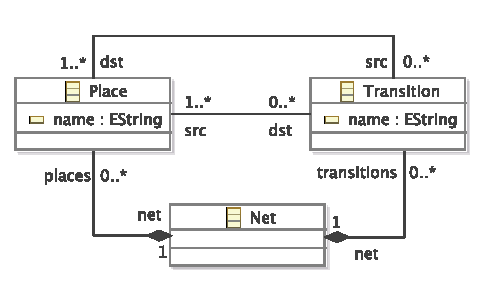
\includegraphics[scale=0.72]{5.Implementation/images/petri_nets_before.pdf}
	}
	\subfigure[Evolved metamodel.]
	{
	    \label{fig:evolved_mm}
	    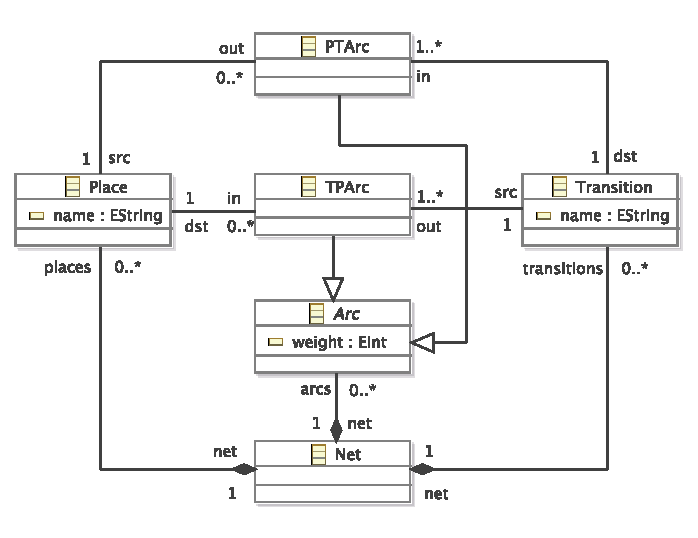
\includegraphics[scale=0.72]{5.Implementation/images/petri_nets_after.pdf}
	}
	\caption[Petri nets metamodel evolution]{Petri nets metamodel evolution. Taken from \cite{rose10flock}.}
\label{fig:petri_nets_mms}
\end{figure}

Models that conform to the original metamodel might not conform to the evolved metamodel. The following strategy can be used to migrate models:

\begin{enumerate}
	\item For every instance, t, of \texttt{Transition}: 
	\subitem For every \texttt{Place}, s, referenced by the \texttt{src} feature of t: 
	\subsubitem Create a new instance, arc, of \texttt{PTArc}. 
	\subsubitem Set s as the \texttt{src} of arc. 
	\subsubitem Set t as the \texttt{dst} of arc. 
	\subsubitem Add arc to the \texttt{arcs} reference of the \texttt{Net} referenced by t.
	
	\subitem For every \texttt{Place}, d, referenced by the \texttt{dst} feature of t: 
	\subsubitem Create a new instance, arc, of \texttt{TPArc}. 
	\subsubitem Set t as the \texttt{src} of arc. 
	\subsubitem Set d as the \texttt{dst} of arc. 
	\subsubitem Add arc to the \texttt{arcs} reference of the \texttt{Net} referenced by t.
	
	\item And nothing else changes.
\end{enumerate}

\subsection{Languages Currently Used for Model Migration}
\label{subsec:existing_migration_languages}
Using the above example, the languages used by existing approaches for specifying and executing model migration strategies are now compared. From this comparison, the strengths and weakness of each language are highlighted and requirements for a model migration language are synthesised in the sequel.

\subsubsection{Manual Specification with M2M Transformation}
\label{subsubsec:m2m}
Model migration can be specified using M2M transformation. For example, the Petri net migration has been specified in the Atlas Transformation Language (ATL) \cite{jouault05transforming}. This is reproduced in Listing~\ref{lst:atl}. Rules for migrating \texttt{Places} and \texttt{TPArcs} have been omitted for brevity, but are similar to the \texttt{Nets} and \texttt{PTArcs} rules.

Model transformation in ATL is specified using \texttt{rule}s, which transform source model elements (specified using the \texttt{fr\-om} keyword) to target model elements (specified using \texttt{to} keyword). For example, the \texttt{Nets} rule on line 1 of Listing~\ref{lst:atl} transforms an instance of \texttt{Net} from the original (source) model to an instance of \texttt{Net} in the evolved (target) model. The source model element (the variable \texttt{o} in the \texttt{Net} rule) is used to populate the target model element (the variable \texttt{m}). ATL allows rules to be specified as \emph{lazy} (not scheduled automatically and applied only when called by other rules).

\begin{lstlisting}[caption={[Fragment of the Petri nets model migration in ATL]Fragment of the Petri nets model migration in ATL, taken from \cite{rose10flock}}, label=lst:atl, language=ATL]
rule Nets {
	from o : Before!Net
	to m : After!Net ( places <- o.places, transitions <- o.transitions )
}

rule Transitions {
	from o : Before!Transition
	to m : After!Transition (
			name <- o.name,
			"in" <- o.src->collect(p | thisModule.PTArcs(p,o)),
			out  <- o.dst->collect(p | thisModule.TPArcs(o,p))
		)
}

unique lazy rule PTArcs {
	from place : Before!Place, destination : Before!Transition
	to ptarcs : After!PTArc (
			src <- place, dst <- destination, net <- destination.net
		)
}
\end{lstlisting}

The \texttt{Transitions} rule in Listing~\ref{lst:atl} codifies in ATL the migration strategy described previously. The rule is executed for each \texttt{Transition} in the original model, \texttt{o}, and constructs a \texttt{PTArc} (\texttt{TPArc}) for each reference to a \texttt{Place} in \texttt{o.src} (\texttt{o.dst}). Lazy rules must be used to produce the arcs to prevent circular dependencies with the \texttt{Transitions} and \texttt{Places} rules. Here, ATL, a typical rule-based transformation language, is considered and model migration would be similar in QVT. With Kermeta, migration would be specified in an imperative style using statements for copying \texttt{Net}s, \texttt{Place}s and \texttt{Transition}s, and for creating \texttt{PTArc}s and \texttt{TPArc}s.

In model transformation, \cite{czarnecki06survey} identifies two common categories of relationship between source and target model, \emph{new-target} and \emph{existing-target}. In the former, the target model is constructed afresh by the execution of the transformation, while in the latter, the target model contains the same data as the source model before the transformation is executed. M2M transformation languages typically support new-target transformations. Some M2M transformation languages also support existing-target transformations, but typically require the source and target metamodel to be identical.

In model migration, source and target metamodels differ, and therefore existing-target transformations cannot be used to specify model migration strategies. Consequently, model migration strategies are specified with new-target model-to-model transformation languages, and often contain sections for copying from original to migrated model those model elements that have not been affected by metamodel evolution. For the Petri nets example, the \texttt{Nets} rule (in Listing~\ref{lst:atl}) and the \texttt{Places} rule (not shown) exist only for this reason.


\subsubsection{Manual Specification with a Metamodel Mapping}
\label{subsubsec:ecore2ecore}
Model migration can be undertaken using the model loading mechanisms of EMF \cite{hussey06advanced}, with a tool that is termed \emph{Ecore2Ecore} here. EMF binds models to a specific metamodel, and hence cannot be used to load models that have been affected by metamodel evolution (Section~\ref{subsec:modelling_framework_characteristics}). Therefore, Ecore2Ecore requires the metamodel developer to provide a mapping between the metamodelling language of EMF (Ecore) and the concrete syntax used to persist models (XMI). Mappings are specified using Ecore2Ecore, which can suggest relationships between source and target metamodel elements by comparing names and types. Figure~\ref{fig:petri_nets_ecore2ecore} shows mappings between the original and evolved Petri nets metamodels.

\begin{figure}[htb]
	\centering
		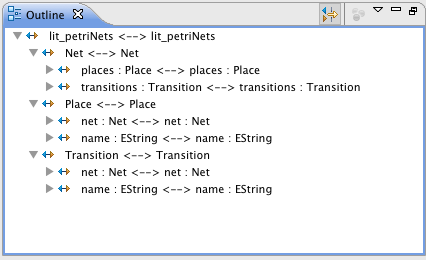
\includegraphics[scale=0.75]{5.Implementation/images/petri_nets_ecore2ecore.png}
	\caption[Mappings between the original and evolved Petri nets metamodels]{Mappings between the original and evolved Petri nets metamodels, constructed with the tool described in \cite{hussey06advanced}}
	\label{fig:petri_nets_ecore2ecore}
\end{figure}


The mappings are used by the EMF XMI parser to determine the metamodel types to which pieces of the XMI will be bound. When a type or feature is not bound, the user must specify a custom migration strategy in Java. For the Petri nets metamodel, the \texttt{src} and \texttt{dst} features of \texttt{Place} and \texttt{Transition} are not bound, because migration is more complicated than a one-to-one mapping.

\begin{lstlisting}[basicstyle=\ttfamily\footnotesize, flexiblecolumns=true, numbers=left, nolol=true, caption=Java method for deserialising a reference., label=lst:java, language=Java, tabsize=2]
private Collection<Place> toCollectionOfPlaces
(String value, Resource resource) {

  final String[] uriFragments    = value.split(" ");
  final Collection<Place> places = new LinkedList<Place>();
 
  for (String uriFragment : uriFragments) {
		final EObject eObject = resource.getEObject(uriFragment);
		final EClass place    = PetriNetsPackage.eINSTANCE.getPlace();

    if (eObject == null || !place.isInstance(eObject))
      // throw an exception
						
		places.add((Place)eObject);
  }
 
  return places;
}
\end{lstlisting}

In Ecore2Ecore, model migration is specified on the XMI representation of the model and requires some knowledge of the XMI standard. For example, in XMI, references to other model elements are serialised as a space delimited collection of URI fragments \cite{steinberg09emf}. Listing~\ref{lst:java} shows a fragment of the code used to migrate Petri net models with Ecore2Ecore. The method shown converts a \texttt{String} containing URI fragments to a \texttt{Collection} of \texttt{Place}s. The method is used to access the \texttt{src} and \texttt{dst} features of \texttt{Tr\-an\-si\-ti\-on}, which no longer exist in the evolved metamodel and hence are not loaded automatically by EMF. To specify the migration strategy for the Petri nets example, the metamodel developer must know the way in which the \texttt{src} and \texttt{dst} features are represented in XMI. The complete listing (presented in Section~\ref{sec:ecore2ecore_listings}) exceeds 150 lines of code.

\subsubsection{Operator-based Co-evolution with COPE}
\label{subsubsec:cope}

Operator-based approaches to identifying and managing co-evolution, such as COPE \cite{herrmannsdoerfer09cope}, provide a library of \emph{co-evolutionary operators}. Each co-evolutionary operator specifies both a metamodel evolution and a corresponding model migration strategy. For example, the ``Make Reference Containment'' operator from COPE \cite{herrmannsdoerfer09cope} evolves the metamodel such that a non-containment reference becomes a containment reference and migrates models such that the values of the evolved reference are replaced by copies. By composing co-evolutionary operators, metamodel evolution can be performed and a migration strategy can be generated without writing any code.

Clearly, the development of an operator-based approach must start by identifying operators, which can be challenging. Operators capture both metamodel evolution and model migration semantics, and as such, a complete library of operators is difficult to imagine \cite{lerner00model}. Instead, operator-based approaches seek to capture the most commonly occurring co-evolutionary operators, which are typically identified by examining existing examples of evolution \cite{herrmannsdoerfer08automatability}. Hence, the breadth of consultation when identifying operators will affect the efficacy of an operator-based approach, because evolutionary changes that occur frequently in one project might never occur in other projects, or vice-versa.

To perform metamodel evolution using an operator-based approach, the library of co-evolutionary operators must be integrated with tools for editing metamodels. COPE provides integration with the EMF tree-based metamodel editor. Operators may be applied to an EMF metamodel, and COPE tracks their application. Once metamodel evolution is complete, a migration strategy can be generated automatically from the record of changes maintained by COPEs. The migration strategy is distributed along with the updated metamodel, and metamodel users choose when to execute the migration strategy on their models.

To be effective, operator-based approaches must provide a rich yet navigable library of co-evolutionary operators (Section~\ref{subsec:co-evolution_categorisation}). COPE allows model migration strategies to be specified manually when no co-evolutionary operator is appropriate. COPE employs a fundamentally different approach to M2M transformation and Ecore2Ecore, using an existing-target transformation. As discussed above, existing-target transformations cannot be used for specifying model migration strategies as the source (original) and target (evolved) metamodels differ. However, models can be structured independently of their metamodel using a metamodel-independent syntax (such as the one introduced in Section~\ref{sec:mmi_syntax}).

Listing~\ref{lst:cope} shows the COPE model migration strategy for the Petri net example given above\footnote{In Listing~\ref{lst:cope}, some of the concrete syntax has been changed in the interest of readability.}. Most notably, slots for features that no longer exist must be explicitly \texttt{unset}. In Listing~\ref{lst:cope}, slots are \texttt{unset} on four occasions (on lines 2, 9, 18 and 19), once for each feature that is in the original metamodel but not in the evolved metamodel. These features are: \texttt{src} and \texttt{dst} of \texttt{Transition} and of \texttt{Place}. Failing to \texttt{unset} slots that do not conform with the evolved metamodel causes migration to fail with an error.

\begin{lstlisting}[caption=Petri nets model migration in COPE, label=lst:cope, language=COPE]
for (transition in petrinets.Transition.allInstances) {
  for (source in transition.unset('src')) {
    def arc = petrinets.PTArc.newInstance()
    arc.src = source
    arc.dst = transition
    arc.net = transition.net
  }
  
  for (destination in transition.unset('dst')) {
    def arc = petrinets.TPArc.newInstance() 
    arc.src = transition
    arc.dst = destination
    arc.net = transition.net
  }
}

for (place in petrinets.Place.allInstances) {
  place.unset('src')
  place.unset('dst')
}
\end{lstlisting}

\subsection{Requirements Identification}
\label{subsec:analysis}
Requirements for a domain-specific for model migration were identified from the review of existing languages (Section~\ref{subsec:existing_migration_languages}). The derivation of the requirements is now summarised, by considering two orthogonal concerns: the source-target relationship of the language used for specifying migration strategies and the way in which models are represented during migration. %and the structures provided by the language for specifying and re-using migration strategies.


\subsubsection{Source-Target Relationship Requirements}
When migration is specified as a new-target transformation, as in ATL (Listing~\ref{lst:atl}), model elements that have not been affected by metamodel evolution must be explicitly copied from the original to the migrated model. When migration is specified as an existing-target transformation, as in COPE (Listing~\ref{lst:cope}), model elements and values that no longer conform to the target metamodel must be explicitly removed from the migrated model. Ecore2Ecore does not require explicit copying or unsetting code; instead, the relationship between original and evolved metamodel elements is captured in a mapping model specified by the metamodel developer. The mapping model can be derived automatically and customised by the metamodel developer. To explore the appropriateness for model migration of an alternative to new- and existing-target transformations, the following requirement was derived:

\emph{The migration language must \textbf{automatically} copy every model element that conforms to the evolved metamodel from original to migrated model, and must automatically not copy any model element that does not conform to the evolved metamodel from original to migrated model.}


\subsubsection{Model Representation Requirements}
With Ecore2Ecore, migration is achieved by manipulating XMI. Consequently, the metamodel developer must be familiar with XMI and must perform tasks such as dereferencing URI fragments (Listing~\ref{lst:java}) and type conversion. Transformation languages abstract over the underlying storage representation of models (such as XMI) by using a modelling framework to load, store and access models.

\emph{The migration language must not expose the underlying representation of models.}

\vspace{5mm}

To apply co-evolution operators, COPE requires the metamodel developer to use a specialised metamodel editor. The editor can manipulate only metamodels defined with EMF. Similarly, the mapping tool used in the Ecore2Ecore approach can be used only with metamodels defined with EMF. Although EMF is arguably very widely-used, other modelling frameworks exist. Adapting to interoperate with new systems is recognised as a common reason for software evolution \cite{sjoberg93quantifying}, and migration between modelling frameworks is as a possible use case for a model migration language. In particular, there is demand for migrating between UML 1 (e.g. \cite{uml14}) and UML 2 (e.g. \cite{uml22}) models\footnote{Forum discussion with Tom Morris, lead developer of the ArgoUML tool, \url{http://www.planet-research20.org/ttc2010/index.php?option=com_community&view=groups&task=viewdiscussion&groupid=4&topicid=20&Itemid=150} (registration required).}, which are typically managed with different modelling frameworks. Decoupling model management operations from the model representation facilitates interoperability with many modelling technologies, as demonstrated by Epsilon (Section~\ref{subsec:epsilon}). Therefor, to faciliate interoperability with modelling frameworks other than EMF, the following requirement was derived:

\emph{The migration language must be loosely coupled with modelling frameworks and must not assume that models and metamodels will be represented in EMF.}
\lstdefinelanguage{Flock}
{morekeywords={for, import, migrate, to, when, original, migrated, typeOf, kindOf, do, not, in, and, or, operation, return, var, if, new, else, delete},
sensitive=true,
morecomment=[l]{--},
morestring=[b]',
showstringspaces=false,
}


\section{Chapter Summary}
Three structures for identifying and managing co-evolution have been designed and implemented to approach the thesis requirements outlined in Chapter~\ref{Analysis}. The way in which modelling frameworks implicitly enforce conformance makes managing non-conformant models challenging, and the proposed metamodel-independent syntax (Section~\ref{sec:mmi_syntax}) extends modelling frameworks to facilitate the management of non-conformant models. The proposed textual modelling notation, Epsilon HUTN (Section~\ref{sec:notation}), provides a human-usable notation as an alternative to XMI for performing user-driven co-evolution. Finally, Epsilon Flock (Section~\ref{sec:flock}) contributes a domain-specific language for describing model migration.

The metamodel-independent syntax is a modelling framework extension that makes explicit the conformance relationship between models and metamodels. By binding models not to their metamodel but to a generic metamodel, the metamodel-independent syntax allows non-conformant models to be managed with modelling tools and model management operations. Furthermore, conformance checking is provided as a service, which can be scheduled at any time, and not just when models are loaded. The metamodel-independent syntax has been integrated with Concordance \cite{rose10concordance} to provide a metamodel installation process that automatically reports conformance problems, and underpins the implementation of the second structure described in this chapter, a textual modelling notation.

For performing user-driven co-evolution, the textual modelling notation described in Section~\ref{sec:notation} provides an alternative to XMI. Unlike XMI, the notation introduced in this chapter implements the OMG standard for Human-Usable Textual Notation (HUTN) \cite{hutn} and is optimised for human usability. Epsilon HUTN, introduced here, is presently the sole reference implementation of HUTN. Constructing Epsilon HUTN by reusing the metamodel-independent syntax allows Epsilon HUTN to provide incremental and background conformance checking, and an XMI-to-HUTN transformation for loading non-conformant models. Section~\ref{sec:exemplar_user-driven_co-evo} explores the benefits and drawbacks of using the metamodel-independent syntax and Epsilon HUTN together to perform user-driven co-evolution.

The domain-specific language described in Section~\ref{sec:flock}, Epsilon Flock, combines several concepts from existing model-to-model transformation languages to form a language tailored to model migration. In particular, Flock contributes a novel mechanism for relating source and target model elements termed conservative copy, which is a hybrid of new- and existing-target styles of model-to-model transformation. Flock extends and reuses Epsilon and hence interoperates transparently with several modelling technologies via EMC, the Epsilon Model Connectivity layer. 

The metamodel-independent syntax, Epsilon HUTN, Epsilon Flock and Concordance have been released as part of Epsilon in the Eclipse GMT\footnote{\url{http://www.eclipse.org/gmt}} project, which is the research incubator of arguably the most widely used MDE modelling framework, EMF. By re-using parts of Epsilon, the structures were implemented more rapidly than would have been possible when developing the structures independently. In particular, re-using EMC facilitated interoperability of Flock with several MDE modelling frameworks, which was exploited to manage a practical case of model migration in Section~\ref{sec:ttc}.